\documentclass[10pt]{article}
\usepackage[letterpaper,margin=1in]{geometry}
\usepackage[T1]{fontenc}
\usepackage{amsmath}
\usepackage{newtxtext,newtxmath}
\usepackage{microtype}
\usepackage{booktabs,array}
\usepackage{graphicx}
\usepackage[round,sort]{natbib}
\usepackage{xcolor}
\usepackage[colorlinks,linkcolor=blue!45!black,citecolor=blue!45!black,urlcolor=blue!45!black]{hyperref}
\usepackage[font=small,labelfont=bf]{caption}
\usepackage{enumitem}
\usepackage{float}
\usepackage{tikz}
\usetikzlibrary{arrows.meta}
\setlist{nosep,leftmargin=1.4em}
\setlength{\parskip}{0.45em}
\setlength{\parindent}{0pt}
\renewcommand{\arraystretch}{1.08}
\newcommand{\phat}{\hat{p}}
\newcommand{\qhat}{\hat{q}}
\newcommand{\blk}[1]{\textsf{\small #1}}

\begin{document}

\begin{center}
{\LARGE\bfseries Predicting Rule Violations Before Generation:\\[3pt] Hidden-State and Attention Probes versus\\[3pt] Prompt-Only Baselines on a Controlled\\[3pt] Multi-Instruction Benchmark\par}
\vspace{0.9em}
{\large Anonymous authors}\\[2pt]
{\normalsize Project report, draft of 16 November 2026}
\end{center}
\vspace{0.3em}

\noindent\fcolorbox{black!35}{black!4}{\parbox{\dimexpr\linewidth-2\fboxsep-2\fboxrule}{\small
\textbf{Status of this draft.} Data generation, verification, feature extraction, model selection and the final model
fits are complete. The analysis plan is frozen. \textbf{The 15 held-out test groups have not been read}, so this
draft contains no test results. Every result in Section~\ref{sec:results} comes from the 57 training groups, either as
a grouped cross-validation loss or from out-of-fold predictions. Section~\ref{sec:next} describes the confirmatory
evaluation and the other work that remains.}}

\begin{abstract}
\noindent Large language models often break some of the instructions in a prompt when several are given at once. We ask
whether such violations can be predicted before the model writes anything, and whether the model's own internal state
at the end of the prompt predicts them better than the prompt text does. We build a controlled dataset from ManyIFEval:
all 216 tasks, 72 groups of three tasks that share a pool of six sampled rules, and a balanced design over rule subsets
($k=1$ to $5$) and rule orders, giving 53,136 prompts. Two 8B generators (Llama~3.1 and Qwen3) each produce 20 responses
per prompt (2.1 million responses in total), checked rule by rule with the official verifiers to give per-rule and
per-prompt violation probabilities. For each generator and objective we compare 23 predictors (hidden-state probes, an
attention-to-rule-span probe, a frozen and a fine-tuned text-encoder baseline, and their combinations) against
structure-only references. The analysis plan is frozen and the test groups are still unread. In grouped
cross-validation on the training groups, the attention probe is the best single predictor of per-rule violations for
both generators (out-of-fold AUROC 0.85 and 0.84, against 0.79 and 0.77 for the fine-tuned text baseline). Probes built
on internal states lower the loss of the strongest comparator without internal access by 8 to 14\% in three of the four
generator--objective cells. In the fourth (per-prompt prediction for Llama) the fine-tuned text baseline matches them.
We also find that the official ``all uppercase'' verifier labels uppercase English as non-English, which accounts for
43\% of Qwen's violations of that rule. We describe the confirmatory test evaluation, the controlled analyses and the
decisions that remain.
\end{abstract}

% ---------------------------------------------------------------------------------------------------------------
\section{Introduction}

People rarely give a language model one instruction. A typical prompt asks for a task and then adds constraints on
length, format, wording and style. Compliance drops as constraints accumulate: on ManyIFEval the share of responses
that follow every instruction falls steadily as the number of instructions grows from one to ten
\citep{harada2025instructions}, and the same pattern holds at much larger instruction counts
\citep{jaroslawicz2025many}. The failure is also silent. A user learns that a rule was broken only after the response
has been generated and checked.

If the probability that each rule will be violated could be estimated \emph{before} generation, a system could act on
it: reorder or restate a risky rule, route the prompt to a stronger model, or sample more candidates. Two sources of
information are available at that point. The first is the prompt itself, which any external model can read. The second
is the generating model's own internal state after it has read the prompt. Work on probing shows that hidden states
carry information about whether an answer will be correct \citep{azaria2023internal,kadavath2022know,orgad2025llms} and
about whether an instruction will be followed \citep{heo2025know}, and that attention to constraint tokens tracks
whether a constraint is satisfied \citep{yuksekgonul2024attention}.

What is less clear is how much of this is specific to the model's internals. Whether a rule is violated depends
strongly on what the rule is. A rule that asks for exactly three paragraphs fails far more often than one that asks for
lowercase letters, and both facts can be read off the prompt. A probe on hidden states may therefore do well simply
because the prompt is encoded in them. The question that matters for practice is the incremental one: does internal
state predict violations better than a strong predictor that sees only the prompt?

This project is designed to answer that question for prompts with several simultaneous rules. We pose four research
questions:
\begin{description}[leftmargin=3.2em,labelwidth=2.6em,labelsep=0.6em,font=\normalfont\bfseries]
\item[RQ1] \textbf{Per-rule violations.} Do pre-generation hidden-state and attention features of the generating model
predict the violation probability of each rule better than prompt-only baselines?
\item[RQ2] \textbf{Overall violations.} Do they predict the expected fraction of a prompt's rules that will be violated
better than those baselines?
\item[RQ3] \textbf{Incremental information.} Do they add predictive value once the prompt text, the exact rule text and
structured prompt properties are already given to the predictor?
\item[RQ4] \textbf{Exact-rule conditioning.} Does giving a hidden-state probe an embedding of the exact rule text
improve it?
\end{description}

Four design choices follow from the question. (i)~Labels are probabilities, estimated from 20 sampled responses per
prompt, because a single response is a noisy outcome. (ii)~The prompts form a balanced design in which the rule set, the
rule order, the number of rules and the task vary one at a time, so that we can later test whether a predictor tracks
the effect of each change. (iii)~Data are split by group of related prompts, never by prompt. (iv)~The prompt-only
baselines are strong: they receive the full prompt text, the exact rule text and structured features, and one of them
fine-tunes its text encoder on the same supervision as the probes.

\paragraph{Contributions and status.}
\begin{itemize}
\item \textbf{A controlled dataset.} 53,136 prompts built from all 216 ManyIFEval tasks, with 2.1 million verified
responses from two generators, per-rule and per-prompt violation probabilities, and pre-generation hidden states and
rule-span attention for every prompt (Section~\ref{sec:data}).
\item \textbf{A pre-specified comparison.} 23 predictor configurations for each of two objectives and two generators,
selected by grouped cross-validation on training groups only, with the analysis plan (metrics, 37 contrasts per cell,
multiple-comparison handling, controlled analyses) frozen and hashed before the test groups are read
(Sections~\ref{sec:predictors} and~\ref{sec:protocol}).
\item \textbf{Training-set evidence.} In cross-validation, the attention probe is the best single per-rule predictor
for both generators, internal-state probes beat prompt-only comparators in three of four cells, and a fine-tuned text
encoder matches them in the fourth (Section~\ref{sec:results}).
\item \textbf{A verifier finding.} The official ``all uppercase'' check fails correct uppercase English responses
because of its language-detection step. This affects 6.1\% of Qwen's checks of that rule (Section~\ref{sec:audit}).
\end{itemize}
What remains is the confirmatory evaluation on the 15 held-out groups, the controlled analyses, and two decisions to be
taken before unblinding (Section~\ref{sec:next}).

% ---------------------------------------------------------------------------------------------------------------
\section{Related work}

\paragraph{Following several instructions at once.} IFEval introduced instructions whose compliance can be verified by
a program, such as word counts, required keywords and formatting \citep{zhou2023ifeval}. ManyIFEval reuses 15 of those
instruction types and combines up to ten in one prompt, showing that compliance degrades with the number of
instructions and that benchmark-level performance on unseen combinations can be estimated from the instruction count
\citep{harada2025instructions}. FollowBench \citep{jiang2024followbench} and InFoBench \citep{qin2024infobench} measure
multi-constraint following with finer-grained requirements, and IFScale scales the count to hundreds of keyword
instructions \citep{jaroslawicz2025many}. These works measure or estimate aggregate compliance. We instead predict, for
one prompt and one rule, the probability that the rule will be violated, and we use ManyIFEval's released rules and
verifiers as the source of ground truth.

\paragraph{Probing internal states for correctness.} Linear and shallow probes on hidden states are a standard tool for
asking what a representation encodes \citep{alain2016probes,belinkov2022probing}, with the known caveat that a probe may
learn the task itself rather than reveal the representation \citep{hewitt2019control}. Probes have been used to detect
whether a statement is true \citep{azaria2023internal,burns2023discovering,marks2024geometry}, whether a model knows an
answer \citep{kadavath2022know}, how uncertain a generation is \citep{kossen2024sep} and what kinds of error a model
will make \citep{orgad2025llms}. KEEN estimates how much a model knows about an entity from its internal
representation before any token is generated \citep{gottesman2024estimating}. Our setting is also pre-generation, but
the target is compliance with explicit constraints, not factual correctness.

\paragraph{Internal states and instruction following.} The closest work is \citet{heo2025know}, who find a direction in
the input embedding space that predicts whether a response will follow a single IFEval instruction, show that it
generalises across tasks but not across instruction types, and use it to steer the model. \citet{stolfo2025steering}
derive steering vectors for format, length and word-inclusion instructions from activation differences. Our study
differs in three ways: prompts contain several rules and each rule is a separate prediction target; labels are
probabilities from repeated sampling; and the probes are compared against prompt-only baselines that receive the same
supervision, which is what determines whether the internal signal is incremental.

\paragraph{Attention as a signal.} \citet{yuksekgonul2024attention} treat a factual query as a set of constraints and
show that attention to constraint tokens predicts whether the constraints are satisfied (SAT Probe). Our attention
probe applies the same idea to instruction spans. Attention to parts of the input also relates to instruction following
through position effects in long contexts \citep{liu2024lost} and through attention steering that emphasises
user-marked spans \citep{zhang2024pasta}. We use attention only as a predictive feature. We make no claim that it
explains the model's behaviour, a distinction the literature has debated \citep{jain2019attention,wiegreffe2019attention}.

% ---------------------------------------------------------------------------------------------------------------
\section{Problem setup}
\label{sec:setup}

A prompt $x$ consists of a task description and an ordered list of $k \le 5$ rules $(r_1,\dots,r_k)$. A generator $G$
samples a response $y \sim G(\cdot \mid x)$, and a deterministic verifier returns $c_r(y)\in\{0,1\}$ for each rule, with
$1$ meaning violated. The quantities of interest are properties of the response distribution:
\[
p_r(x) = \Pr_{y\sim G(\cdot\mid x)}\!\left[c_r(y)=1\right], \qquad q(x) = \frac{1}{k}\sum_{j=1}^{k} p_{r_j}(x).
\]
We estimate them from $n=20$ independent samples per prompt: $\phat_r(x) = v_r(x)/n$, where $v_r$ is the number of
sampled responses that violate $r$, and $\qhat(x)$ is the mean of $\phat$ over the prompt's rules. Note that $q$ is the
expected \emph{fraction} of rules violated, not the probability that at least one is.

\textbf{Objective~1} is to predict $p_r(x)$ for every (prompt, rule) pair. \textbf{Objective~2} is to predict $q(x)$
for every prompt. Every predictor may use only information that exists before the first response token: the prompt
text, its known structure, and the generator's activations on the prompt. Sampled responses and verifier outputs are
used only as labels. The two generators are treated as separate experiments. Each has its own responses, labels,
internal features and fitted predictors, and nothing is pooled across them.

% ---------------------------------------------------------------------------------------------------------------
\section{Dataset}
\label{sec:data}

\begin{figure}[t]
\centering
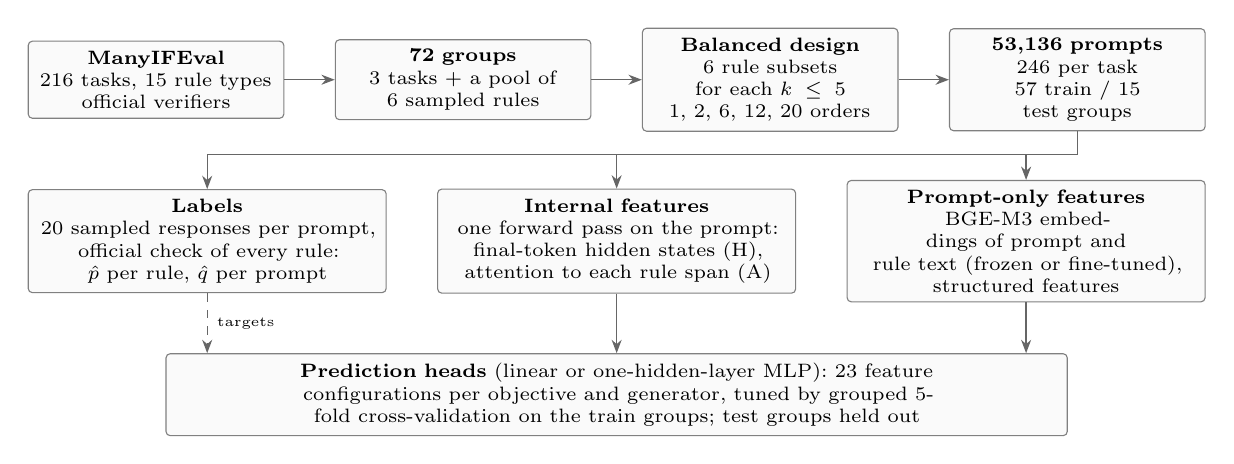
\begin{tikzpicture}[font=\scriptsize,
  box/.style={draw=black!50, rounded corners=1.5pt, align=center, inner sep=3.5pt, text width=#1, fill=black!2},
  box/.default=3.0cm, arr/.style={-{Stealth[length=1.7mm]}, draw=black!60, line width=0.5pt}]
\node[box] (src) at (0,0) {\textbf{ManyIFEval}\\216 tasks, 15 rule types\\official verifiers};
\node[box] (grp) at (3.9,0) {\textbf{72 groups}\\3 tasks + a pool of\\6 sampled rules};
\node[box] (des) at (7.8,0) {\textbf{Balanced design}\\6 rule subsets for each $k\le5$\\1, 2, 6, 12, 20 orders};
\node[box] (pr) at (11.7,0) {\textbf{53,136 prompts}\\246 per task\\57 train / 15 test groups};
\draw[arr] (src) -- (grp); \draw[arr] (grp) -- (des); \draw[arr] (des) -- (pr);
\node[box=4.3cm] (lab) at (0.65,-2.05) {\textbf{Labels}\\20 sampled responses per prompt,\\official check of every rule:\\$\phat$ per rule, $\qhat$ per prompt};
\node[box=4.3cm] (int) at (5.85,-2.05) {\textbf{Internal features}\\one forward pass on the prompt:\\final-token hidden states (H),\\attention to each rule span (A)};
\node[box=4.3cm] (txt) at (11.05,-2.05) {\textbf{Prompt-only features}\\BGE-M3 embeddings of prompt and\\rule text (frozen or fine-tuned),\\structured features};
\coordinate (bus) at (11.7,-0.95);
\draw[draw=black!60, line width=0.5pt] (pr.south) -- (bus);
\draw[arr] (bus) -| (lab.north); \draw[arr] (bus) -| (int.north); \draw[arr] (bus) -| (txt.north);
\node[box=11.2cm] (hd) at (5.85,-4.0) {\textbf{Prediction heads} (linear or one-hidden-layer MLP): 23 feature configurations
per objective and generator, tuned by grouped 5-fold cross-validation on the train groups; test groups held out};
\draw[arr] (int.south) -- (int.south |- hd.north); \draw[arr] (txt.south) -- (txt.south |- hd.north);
\draw[arr, dashed] (lab.south) -- (lab.south |- hd.north) node[midway, right, font=\tiny] {targets};
\end{tikzpicture}
\caption{Overview. Prompts are built from ManyIFEval tasks and rules in a balanced design. Each generator supplies
labels (from sampled responses) and internal features (from one forward pass on the prompt alone). Predictors that use
internal features are compared with predictors that see only the prompt.}
\label{fig:overview}
\end{figure}

\subsection{Source, groups and rule pools}

\textbf{Source.} We use the released ManyIFEval repository \citep{harada2025instructions} at a pinned commit: its 216
task descriptions, its 15 instruction types (Appendix~\ref{app:types}) and the official verifier of each type, which
come from IFEval \citep{zhou2023ifeval}. Before building anything, we check that our prompt serialiser reproduces all
2,160 released ManyIFEval prompts byte for byte.

\textbf{Groups.} All 216 tasks are used. We assigned each task one of six family labels (informational, creative,
persuasive, practical, analytical, transformation) from its text, following a written rubric. These labels are our
proposal, not part of ManyIFEval. The tasks are then formed into 72 groups of three, each group drawing from three
different families.

\textbf{Rule pools.} Each group receives its own pool of six rules with six distinct types. Types are proposed
uniformly at random and accepted if the pool can still be completed with compatible types. Two types are incompatible
if they belong to the same mutually exclusive set: \{keyword existence, keyword frequency\}, the three letter-case
types, or \{word count, sentence count, paragraph count\}. This rule reproduces every type combination in the released
data. Rule parameters are drawn by calling the released instruction classes with their default generators, so the
released code alone defines the parameter ranges. A draw is rejected only if it is provably unsatisfiable or
contradicts another rule in the pool, and a pool is accepted only when a constructed witness response passes all six
official verifiers for each of the group's three tasks. One parameter draw was rejected in the whole build. There is no
filter for how natural a rule is for a task. The result is 432 rule instances, fixed within their group and sampled
independently across groups.

\subsection{Rule subsets and orders}

Within a group, the six rules are placed in one random cyclic order. Each of the six rotations of that order, cut to
five rules, is a \emph{chain}, and the first $k$ rules of a chain form a rule subset for $k=1,\dots,5$. This gives six
subsets at every $k$, with every rule in exactly $k$ of them, and subsets that are nested along a chain, so that adding
one rule to a prompt is a controlled change. Each subset is presented in 1, 2, 6, 12 or 20 orders for $k=1,\dots,5$,
taken from a strength-two component orthogonal array \citep{yang2021coa}: for $k\ge2$ every rule appears in every
position equally often, and every ordered pair of rules appears at every pair of positions exactly once. The design
does not cover all $k!$ orders for $k\ge4$. In total each task receives 246 ordered rule lists, and the same 246 lists
are applied to all three tasks of the group. A prompt is the task text followed by ManyIFEval's fixed header and one
bullet per rule (example in Appendix~\ref{app:types}).

\begin{table}[t]
\centering\small
\caption{Dataset size. Responses are per generator. Prompt--rule rows are the units of Objective~1 and prompts the
units of Objective~2.}
\label{tab:counts}
\begin{tabular}{lrrrrr}
\toprule
 & Per task & Per group & Train & Test & All \\
\midrule
Groups & & 1 & 57 & 15 & 72 \\
Tasks & 1 & 3 & 171 & 45 & 216 \\
Prompts & 246 & 738 & 42,066 & 11,070 & 53,136 \\
Prompt--rule rows & 1,026 & 3,078 & 175,446 & 46,170 & 221,616 \\
Responses (per generator) & 4,920 & 14,760 & 841,320 & 221,400 & 1,062,720 \\
\bottomrule
\end{tabular}
\end{table}

\subsection{Split}

Groups are the unit of independence, because the prompts of a group share tasks, rules and orders. We hold out 15 of
the 72 groups as the test set and keep 57 for training (Table~\ref{tab:counts}). There is no separate validation set.
The split was chosen before any response was generated, by scoring 20,000 random candidate splits on how closely the
test set's mix of task families and rule types matches the whole dataset, subject to every rule type appearing in at
least one test group and at least five training groups. Eight clusters of near-duplicate tasks are kept on the same
side. Because rule pools are sampled independently, 50 of the 90 test rule instances coincide in type and parameters
with some training rule (the five parameter-free types always do). The test set therefore measures generalisation to
unseen tasks and unseen rule combinations, not to unseen rule wordings.

\subsection{Responses, verification and labels}

\textbf{Generators.} \texttt{meta-llama/Llama-3.1-8B-Instruct} \citep{grattafiori2024llama3} and
\texttt{Qwen/Qwen3-8B} \citep{yang2025qwen3} with thinking disabled, both at pinned revisions and unquantised (bfloat16).
Each prompt is a single user turn rendered with the model's chat template. We sample 20 responses per prompt with each
model card's default decoding settings (Llama: temperature 0.6, top-$p$ 0.9; Qwen: temperature 0.7, top-$p$ 0.8,
top-$k$ 20) and a limit of 2,048 new tokens, using vLLM \citep{kwon2023vllm} on NVIDIA B200 GPUs. No prompt is
truncated (the longest is 216 tokens).

\textbf{Verification.} Every rule in the prompt is checked on every response with the official verifier. A rule counts
as followed only if the response is non-empty and the check passes. The verifier's two sources of nondeterminism
(language detection and sentence splitting) are seeded or pinned, so labels are reproducible. Nothing is dropped:
responses that hit the token limit or fall into repetition loops stay in the labels, and we report how common they
are.

\subsection{Pre-generation features}
\label{sec:features}

For each prompt and generator we run one forward pass on the rendered prompt alone and read everything at the
\emph{final prompt token}, the position from which the first response token is sampled. We store (a)~the
4,096-dimensional hidden state at that token after every layer, and (b)~for every layer and attention head
($32\times32$ for Llama, $36\times32$ for Qwen), the attention weight from that token to the exact token span of each
rule, both summed over the span and averaged over it. These features are computed with Hugging Face Transformers on
Apple silicon, a different backend from the one that generated the responses. A pilot comparison found hidden-state
cosine similarity of at least 0.998 between backends, so the stored states approximate the generating states closely
but not exactly. All features come from one backend and are never mixed.

% ---------------------------------------------------------------------------------------------------------------
\section{Predictors}
\label{sec:predictors}

\subsection{Five components}

Each predictor is a small head on a concatenation of feature blocks. The blocks come from five components
(Table~\ref{tab:components}). Three use the generator's internals:
\begin{itemize}
\item \textbf{H1}, the hidden state at the final prompt token at one layer.
\item \textbf{H2}, the same hidden state together with a text embedding of the exact rule.
\item \textbf{A1}, the attention from the final prompt token to the target rule's span, one value per layer and head.
\end{itemize}
Two see only the prompt:
\begin{itemize}
\item \textbf{B1}, embeddings of the full prompt and of the rule text from a frozen BGE-M3 encoder
\citep{chen2024bge}, plus structured features.
\item \textbf{B2}, the same inputs with the encoder fine-tuned on the prediction task.
\end{itemize}
The structured features describe the prompt without its wording: $k$, the target rule's type, position and numeric
parameters, which other rule types are present and their parameters, the task family and the prompt length (75 columns
for Objective~1, 175 for Objective~2). Exact rule identifiers, group identifiers and task identifiers are never inputs.

\begin{table}[t]
\centering\small
\caption{The five components and the feature blocks they contribute. \blk{H}: hidden state (4,096). \blk{A}: attention
to the target rule span (1,024 for Llama, 1,152 for Qwen). \blk{A5}: attention to up to five rule slots in prompt order
with a presence mask. \blk{EP}, \blk{ER}: BGE-M3 embeddings of the prompt and of the target rule (1,024 each).
\blk{ER5}: rule embeddings in five ordered slots. \blk{S1}, \blk{S2}: structured features. \blk{M2}: rule types and
order only (a subset of \blk{S2}). \blk{KM}: $k$ only. The subscript B2 marks the fine-tuned encoder.}
\label{tab:components}
\begin{tabular}{llll}
\toprule
Component & Uses internals & Objective~1 (per prompt--rule) & Objective~2 (per prompt) \\
\midrule
H1 & yes & \blk{H} & \blk{H} + \blk{M2} \\
H2 & yes & \blk{H} + \blk{ER} & \blk{H} + \blk{M2} + \blk{ER5} \\
A1 & yes & \blk{A} & \blk{A5} + \blk{KM} \\
B1 & no & \blk{EP} + \blk{ER} + \blk{S1} & \blk{EP} + \blk{ER5} + \blk{S2} \\
B2 & no & \blk{EP}$_\text{B2}$ + \blk{ER}$_\text{B2}$ + \blk{S1} & \blk{EP}$_\text{B2}$ + \blk{ER5}$_\text{B2}$ + \blk{S2} \\
\bottomrule
\end{tabular}
\end{table}

\subsection{The 23 configurations}

The configurations are the seven non-empty combinations of \{H1, H2, A1\} (``probe-only''), B1 alone and with each of
those seven (``B1 family''), and B2 alone and with each of the seven (``B2 family''): $7+8+8=23$. A combination uses
the union of its components' blocks. Because H1 and H2 share one hidden-state layer and B1 already contains the rule
embedding that H2 adds, some combinations have identical inputs (for example H2 and H1+H2, or B1+H1 and B1+H2). There
are 15 distinct feature sets among the 23 names (Appendix~\ref{app:config}). Differences between configurations with
identical inputs reflect only the random seed of the head.

\textbf{Heads.} For Objective~1, any configuration that contains H1, H2 or A1 uses 15 separate heads, one per rule
type. A prompt--rule row is routed to the head of its rule's type. Parameter variants of a type share a head, and no
exact rule has its own weights. B1 alone, B2 alone and the structure reference use a single shared head, which receives
the rule type as an input feature. For Objective~2 every configuration uses one shared head.

\textbf{References.} Four reference predictors show how far simple information goes: the overall training violation
rate (``constant rate''), the rate of the rule's type (``type rate''), the rate of the type at that $k$ (``type $\times$
$k$ rate''), and a learned head on the structured features alone (``structure head''). The structure head is the
closest comparator for the question ``does anything beyond the prompt's known structure help?''. It knows the rule
types, parameters, positions and task family, but not the wording and not the generator's state.

% ---------------------------------------------------------------------------------------------------------------
\section{Experimental protocol}
\label{sec:protocol}

\textbf{Heads and losses.} Each configuration is fitted with a linear head and with a one-hidden-layer MLP (128 ReLU
units), each at three strengths of an $L_2$ penalty, $\lambda\in\{0.01, 0.1, 1\}$, on standardised features. The output
is a sigmoid. Objective~1 minimises the binomial negative log-likelihood (NLL) of $v$ violations in $n=20$ responses,
reported per (response, rule) check. Objective~2 minimises the squared error against $\qhat$. Standardisation uses the
fitting rows only.

\textbf{Selection by grouped cross-validation.} The 57 training groups are divided once into five folds of 12, 12, 11,
11 and 11 groups. For each configuration, each of the six head settings is fitted on four folds and scored on the
fifth, and the setting with the lowest mean held-out loss is selected. The number of MLP epochs (up to 30) is chosen in
the same way. Two choices are made once per generator and objective and then shared by all configurations: the
hidden-state layer (50\%, 75\% or 100\% of depth, chosen on H1) and the attention pooling over the rule span (sum or
mean, chosen on A1).

\textbf{Fine-tuned baseline (B2).} BGE-M3 is adapted with LoRA \citep{hu2022lora} (rank 16) jointly with a linear head
on the objective's loss, over a grid of two learning rates and one or three epochs, separately inside every fold so
that an encoder never sees its held-out groups (80 runs). The choice of LoRA over full fine-tuning was made by a rule
fixed in advance on one fold. The embeddings of the selected encoder then go through the same head grid as every other
configuration, alone (B2) and combined with each probe.

\textbf{Final models.} Each selected setting is refitted on all 57 training groups. These refitted models are the ones
that will be applied, once, to the test groups.

\textbf{Pre-specification and test-set discipline.} All choices above were made on training data. The analysis plan
(selected settings, metrics, bootstrap procedure, the list of contrasts, multiple-comparison handling, controlled
analyses and sensitivity analyses) was written to a file whose hash is recorded together with hashes of the folds, the
manifest and the configuration. The data loaders refuse to return test rows until unblinding is recorded, an automated
test guards this, and the fine-tuning jobs received a bundle that contained training rows only. One exception is
disclosed: during a data-integrity check before the probing work started, the share of responses that hit the token
limit was computed over all prompts, test groups included. No modelling choice used it.

\textbf{Descriptive analysis of out-of-fold predictions.} Cross-validation leaves, for every training row, a
prediction from a model that did not see that row's group. To express the cross-validation results in interpretable
units we score these out-of-fold (OOF) predictions with the metrics planned for the test set, and attach percentile
intervals from a paired bootstrap that resamples the 57 training groups (2,000 replicates). These intervals describe
variation across training groups. They are not confirmatory: head settings were selected on the same folds, which makes
the selected losses slightly optimistic \citep{cawley2010overfitting}, and this analysis was not part of the frozen plan.
We report no $p$-values for it.

% ---------------------------------------------------------------------------------------------------------------
\section{Results so far (training groups only)}
\label{sec:results}

\subsection{How often rules are violated}

\begin{figure}[t]
\centering
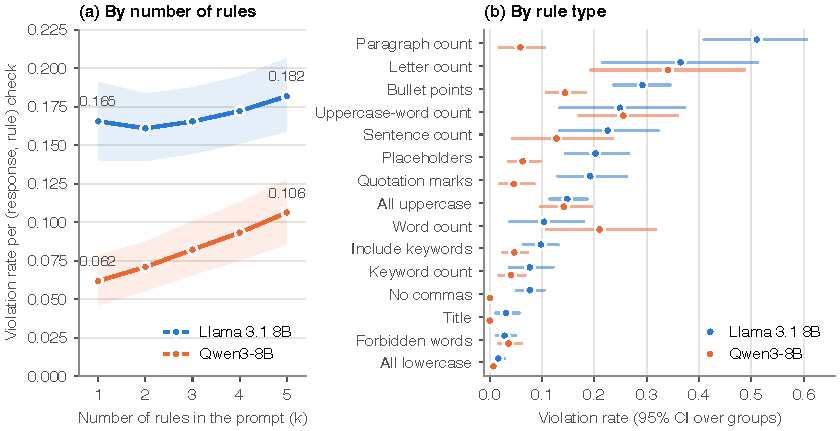
\includegraphics[width=\linewidth]{figures/fig_violation.pdf}
\caption{Violation rates on the training groups. (a)~Share of (response, rule) checks that fail, by number of rules in
the prompt. (b)~The same by rule type. Bands and bars are 95\% intervals from a bootstrap over the 57 groups.}
\label{fig:violation}
\end{figure}

Llama violates 17.7\% of (response, rule) checks (95\% interval 15.5 to 20.0) and Qwen 9.9\% (8.0 to 11.9). The rate
rises with the number of rules for Qwen, from 6.2\% at $k=1$ to 10.6\% at $k=5$, and less clearly for Llama, from
16.5\% to 18.2\% with a dip at $k=2$ (Figure~\ref{fig:violation}a). Rule type matters far more than $k$
(Figure~\ref{fig:violation}b). Paragraph count is violated in 51.1\% of Llama's checks but 5.9\% of Qwen's; letter
count in 36.5\% and 34.1\%; all-lowercase in 1.6\% and 0.7\%.

The aggregate trend in $k$ also hides opposite trends by type (Figure~\ref{fig:typek}, Appendix~\ref{app:desc}).
Qwen's word-count violations rise from 1.1\% at $k=1$ to 23.1\% at $k=5$, while Llama's all-uppercase violations fall
from 22.3\% to 14.4\%. Within a prompt of five rules, Llama's rate rises from 17.7\% for the rule listed first to 18.9\%
for the rule listed last, and Qwen's is flat (10.4\% and 10.5\%). The two generators agree only moderately on which
prompts are hard: the rank correlation of their per-prompt $\qhat$ is 0.43 (0.36 to 0.51).

The labels are skewed. In 53.2\% of Llama's prompt--rule rows and 74.6\% of Qwen's, none of the 20 responses violates
the rule, and in 5.4\% and 3.9\% all 20 do (Table~\ref{tab:quality}, Appendix~\ref{app:desc}). This is why the
objectives are scored with losses on probabilities and why constant and rate-based references are reported throughout.

\subsection{Cross-validated comparison of the 23 configurations}

\begin{table}[t]
\centering\small
\caption{Grouped cross-validation loss on the training groups (mean of five held-out folds; lower is better).
Objective~1: binomial NLL per check. Objective~2: mean squared error in units of $10^{-2}$. Bold marks the lowest loss
in each column. The last two rows give the best combination of a baseline with one or more probes, named in
parentheses. All 23 configurations are in Appendix~\ref{app:fullcv}.}
\label{tab:cv}
% generated by report/make_tables.py -- do not edit
\begin{tabular}{lcccc}
\toprule
 & \multicolumn{2}{c}{Llama 3.1 8B} & \multicolumn{2}{c}{Qwen3-8B} \\
\cmidrule(lr){2-3}\cmidrule(lr){4-5}
Predictor & Obj.~1 NLL & Obj.~2 MSE & Obj.~1 NLL & Obj.~2 MSE \\
\midrule
Constant rate & 0.4705 & 2.364 & 0.3256 & 1.577 \\
Type rate & 0.4155 & 2.046 & 0.2765 & 1.379 \\
Type $\times$ $k$ rate & 0.4152 & 2.036 & 0.2756 & 1.350 \\
Structure head & 0.3779 & 1.847 & 0.2573 & 1.275 \\
\midrule
B1 & 0.3868 & 1.838 & 0.2646 & 1.360 \\
B2 & 0.3700 & 1.613 & 0.2606 & 1.379 \\
\midrule
H1 & 0.3761 & 1.656 & 0.2613 & 1.130 \\
H2 & 0.3390 & 1.643 & 0.2396 & 1.192 \\
A1 & \textbf{0.3316} & 1.693 & 0.2361 & 1.274 \\
H1+A1 & 0.3583 & 1.585 & 0.2556 & \textbf{1.103} \\
H2+A1 & 0.3364 & 1.603 & 0.2386 & 1.164 \\
H1+H2+A1 & 0.3363 & 1.603 & 0.2358 & 1.164 \\
\midrule
Best B1 + probe & 0.3390 {\scriptsize(B1+H1+A1)} & 1.638 {\scriptsize(B1+H1+A1)} & 0.2374 {\scriptsize(B1+H1+H2+A1)} & 1.199 {\scriptsize(B1+H1+A1)} \\
Best B2 + probe & 0.3341 {\scriptsize(B2+H1+H2+A1)} & \textbf{1.562} {\scriptsize(B2+H2+A1)} & \textbf{0.2324} {\scriptsize(B2+H1+H2+A1)} & 1.342 {\scriptsize(B2+H2+A1)} \\
\midrule
Of 23 below structure head & 22 & 23 & 20 & 13 \\
\bottomrule
\end{tabular}

\end{table}

\begin{figure}[t]
\centering
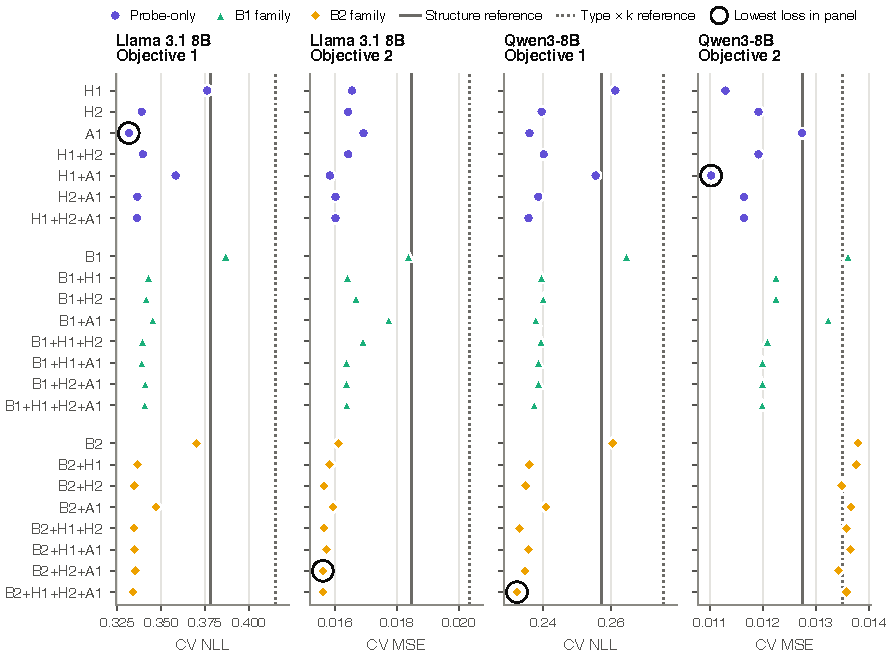
\includegraphics[width=\linewidth]{figures/fig_cv_configs.pdf}
\caption{Cross-validation loss of all 23 configurations in each generator--objective cell. Vertical lines mark the two
strongest references. Configurations with identical inputs (Section~\ref{sec:predictors}) differ only through the
seed of their heads. The horizontal scale differs between panels.}
\label{fig:cv}
\end{figure}

Table~\ref{tab:cv} and Figure~\ref{fig:cv} give the cross-validation losses. Five observations follow.

\textbf{Known structure already explains a lot.} Relative to the constant rate, the type $\times$ $k$ rate lowers the
Objective~1 loss by 11.8\% for Llama and 15.3\% for Qwen, and the structure head by 19.7\% and 21.0\%. Any claim about
internal states has to be made against this level, not against chance.

\textbf{Text embeddings add little to structure.} The frozen text baseline B1 does not improve on the structure head:
its loss is higher in both objectives for Qwen and in Objective~1 for Llama, and only 0.5\% lower in Objective~2 for Llama. Fine-tuning the encoder (B2) helps for Llama in both objectives and does not help for Qwen.

\textbf{Per-rule prediction: attention is the best single signal.} For Objective~1 the attention probe A1 has the
lowest loss of any single component for both generators (0.3316 for Llama and 0.2361 for Qwen), followed by the
rule-conditioned hidden-state probe H2 (0.3390 and 0.2396). The plain hidden-state probe H1 (0.3761 and 0.2613) is no
better than the structure head. The best probe-only configuration lowers the loss of the structure head by 12.3\%
(Llama) and 8.4\% (Qwen), and that of B2 by 10.4\% and 9.5\%. Adding a baseline to the probes changes little: the best
B2-plus-probe combination reaches 0.3341 for Llama (above A1 alone) and 0.2324 for Qwen (the lowest in its column, 1.4\%
below the best probe-only configuration).

\textbf{Per-prompt prediction: the generators differ.} For Qwen, hidden-state probes are clearly best in Objective~2.
H1 reaches 1.130 and H1+A1 1.103, against 1.275 for the structure head and 1.360 and 1.379 for B1 and B2, and adding
probes to B2 does not recover the difference (1.342 at best). For Llama, all learned predictors lie in a narrow band.
B2 alone reaches 1.613, the best probe-only configuration 1.585, and the lowest loss, 1.562, combines B2 with H2 and
A1.

\textbf{Most configurations beat the structure head, except where the baselines drag them down.} 22, 23 and 20 of the
23 configurations have a lower loss than the structure head in the first three columns of Table~\ref{tab:cv}. In
Objective~2 for Qwen only 13 do: the seven probe-only configurations and six of the B1 family, and none of the B2
family.

\subsection{Effect sizes from out-of-fold predictions}

\begin{table}[t]
\centering\small
\caption{The best probe-only configuration of each cell against the three comparators without internal access.
$\Delta$ CV loss: relative change in the cross-validation loss of Table~\ref{tab:cv}. $\Delta$ primary metric:
difference in pooled out-of-fold NLL (Objective~1) or RMSE (Objective~2), probe minus comparator, with a 95\% interval
from a paired bootstrap over the 57 training groups. Folds: held-out folds, of five, in which the probe has the lower
loss. Descriptive, training groups only.}
\label{tab:bestvs}
% generated by report/make_tables.py -- do not edit
\begin{tabular}{lllccc}
\toprule
Cell & Best probe-only & Comparator & $\Delta$ CV loss & $\Delta$ primary metric, OOF [95\% interval] & Folds \\
\midrule
Llama, Obj.~1 & A1 & Structure head & $-12.3\%$ & $-0.0464$ {\scriptsize[$-0.0625$, $-0.0309$]} & 5/5 \\
 &  & B1 & $-14.3\%$ & $-0.0554$ {\scriptsize[$-0.0718$, $-0.0407$]} & 5/5 \\
 &  & B2 & $-10.4\%$ & $-0.0387$ {\scriptsize[$-0.0537$, $-0.0234$]} & 5/5 \\
\midrule
Llama, Obj.~2 & H1+A1 & Structure head & $-14.2\%$ & $-0.0104$ {\scriptsize[$-0.0192$, $-0.0023$]} & 4/5 \\
 &  & B1 & $-13.8\%$ & $-0.0099$ {\scriptsize[$-0.0177$, $-0.0022$]} & 5/5 \\
 &  & B2 & $-1.7\%$ & $-0.0013$ {\scriptsize[$-0.0095$, $+0.0068$]} & 3/5 \\
\midrule
Qwen, Obj.~1 & H1+H2+A1 & Structure head & $-8.4\%$ & $-0.0208$ {\scriptsize[$-0.0367$, $-0.0062$]} & 4/5 \\
 &  & B1 & $-10.9\%$ & $-0.0276$ {\scriptsize[$-0.0456$, $-0.0085$]} & 4/5 \\
 &  & B2 & $-9.5\%$ & $-0.0236$ {\scriptsize[$-0.0427$, $-0.0065$]} & 3/5 \\
\midrule
Qwen, Obj.~2 & H1+A1 & Structure head & $-13.5\%$ & $-0.0079$ {\scriptsize[$-0.0138$, $-0.0025$]} & 4/5 \\
 &  & B1 & $-18.9\%$ & $-0.0114$ {\scriptsize[$-0.0173$, $-0.0066$]} & 5/5 \\
 &  & B2 & $-20.0\%$ & $-0.0124$ {\scriptsize[$-0.0201$, $-0.0053$]} & 5/5 \\
\bottomrule
\end{tabular}

\end{table}

\begin{figure}[t]
\centering
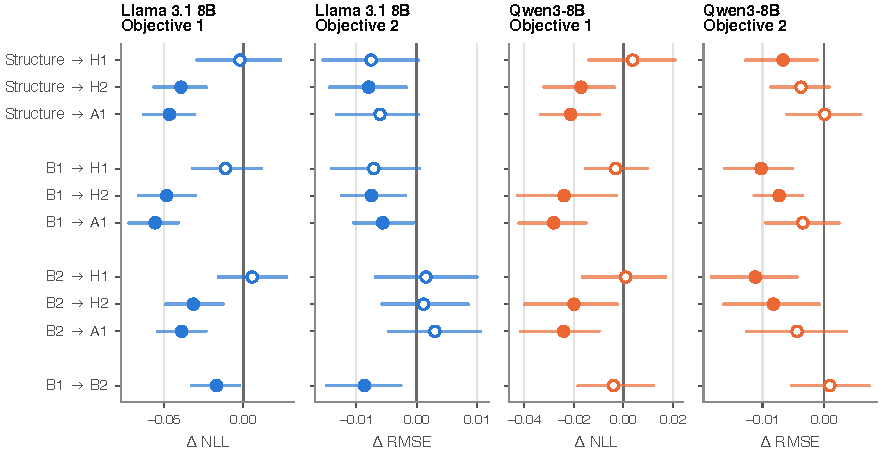
\includegraphics[width=\linewidth]{figures/fig_contrasts.pdf}
\caption{Out-of-fold differences on the training groups for single components: each internal-state probe against the
structure head, B1 and B2, and B2 against B1. Points are the difference in the primary metric (second configuration
minus first, so negative values favour the second), with 95\% intervals from a paired bootstrap over training groups.
Filled points have intervals that exclude zero. Descriptive, not confirmatory.}
\label{fig:contrasts}
\end{figure}

\begin{table}[t]
\centering\small
\caption{Out-of-fold metrics on the training groups, Objective~1 (pooled over the five held-out folds). The interval is
for NLL. Top and bottom 10\%: observed violation rate among the tenth of rows with the highest and lowest predicted
risk.}
\label{tab:oof1}
% generated by report/make_tables.py -- do not edit
\begin{tabular}{llcccccc}
\toprule
 & Predictor & NLL & 95\% interval & Brier & AUROC & Top 10\% & Bottom 10\% \\
\midrule
Llama & Type $\times$ $k$ rate & 0.4150 & {\scriptsize[0.3887, 0.4445]} & 0.1311 & 0.740 & 0.387 & 0.044 \\
 & Structure head & 0.3776 & {\scriptsize[0.3444, 0.4131]} & 0.1180 & 0.809 & 0.572 & 0.026 \\
 & B1 & 0.3867 & {\scriptsize[0.3588, 0.4158]} & 0.1203 & 0.784 & 0.538 & 0.029 \\
 & B2 & 0.3699 & {\scriptsize[0.3405, 0.4020]} & 0.1114 & 0.793 & 0.641 & 0.042 \\
 & H1 & 0.3755 & {\scriptsize[0.3446, 0.4075]} & 0.1158 & 0.808 & 0.595 & 0.015 \\
 & H2 & 0.3385 & {\scriptsize[0.3074, 0.3731]} & 0.1032 & 0.848 & 0.697 & 0.018 \\
 & A1\,{\scriptsize(lowest CV loss)} & 0.3312 & {\scriptsize[0.3024, 0.3640]} & 0.1002 & 0.852 & 0.709 & 0.007 \\
\midrule
Qwen & Type $\times$ $k$ rate & 0.2749 & {\scriptsize[0.2448, 0.3078]} & 0.0814 & 0.784 & 0.301 & 0.001 \\
 & Structure head & 0.2573 & {\scriptsize[0.2198, 0.3004]} & 0.0733 & 0.817 & 0.441 & 0.004 \\
 & B1 & 0.2641 & {\scriptsize[0.2326, 0.2982]} & 0.0751 & 0.792 & 0.376 & 0.002 \\
 & B2 & 0.2601 & {\scriptsize[0.2261, 0.2995]} & 0.0711 & 0.774 & 0.382 & 0.027 \\
 & H1 & 0.2609 & {\scriptsize[0.2314, 0.2953]} & 0.0772 & 0.818 & 0.359 & 0.001 \\
 & H2 & 0.2402 & {\scriptsize[0.2048, 0.2827]} & 0.0687 & 0.849 & 0.461 & 0.001 \\
 & A1 & 0.2360 & {\scriptsize[0.2053, 0.2717]} & 0.0673 & 0.844 & 0.472 & 0.001 \\
 & H1+H2+A1\,{\scriptsize(best probe-only)} & 0.2365 & {\scriptsize[0.2041, 0.2756]} & 0.0679 & 0.856 & 0.470 & 0.001 \\
 & B2+H1+H2+A1\,{\scriptsize(lowest CV loss)} & 0.2328 & {\scriptsize[0.1961, 0.2775]} & 0.0654 & 0.852 & 0.475 & 0.001 \\
\bottomrule
\end{tabular}

\end{table}

Table~\ref{tab:bestvs} compares the best probe-only configuration of each cell with the three comparators, and
Figure~\ref{fig:contrasts} shows the single-component contrasts. In Objective~1 the attention probe lowers the
out-of-fold NLL relative to B2 by 0.039 for Llama (95\% interval 0.023 to 0.054) and by 0.024 for Qwen (0.010 to
0.041), and it has the lower loss in all five folds for both generators. H2 also lowers the NLL relative to B2 for both generators, by slightly less, with intervals that exclude zero. H1 alone cannot be distinguished from the structure head or from B2 in Objective~1: all four
intervals include zero.

In Objective~2 the picture depends on the generator, as in the cross-validation losses. For Qwen, H1 lowers RMSE by
0.010 relative to B1 (0.005 to 0.016) and by 0.011 relative to B2 (0.004 to 0.018). For Llama, no probe differs from
B2: the best probe-only configuration changes RMSE by $-0.001$ ($-0.010$ to $+0.007$).

In terms of ranking (Table~\ref{tab:oof1}), A1 separates violated from followed checks with an out-of-fold AUROC of
0.852 for Llama and 0.844 for Qwen, against 0.793 and 0.774 for B2 and 0.809 and 0.817 for the structure head. Among
the tenth of Llama's prompt--rule rows that A1 rates as riskiest, 70.9\% of checks are violated, against 57.2\% for the
structure head, and among the tenth it rates as safest, 0.7\% against 2.6\%. For Objective~2
(Table~\ref{tab:oof2}, Appendix~\ref{app:oof}), the rank correlation between predicted and observed $\qhat$ for the
best probe-only configuration is 0.55 for Llama and 0.50 for Qwen, against 0.47 and 0.42 for the structure head.
Predictions are close to calibrated out of fold: expected calibration error \citep{guo2017calibration} in decile bins
is below 0.03 for every Objective~1 predictor in Table~\ref{tab:oof1} (Figure~\ref{fig:reliability},
Appendix~\ref{app:oof}).

\subsection{Where the internal signal helps}

\begin{figure}[t]
\centering
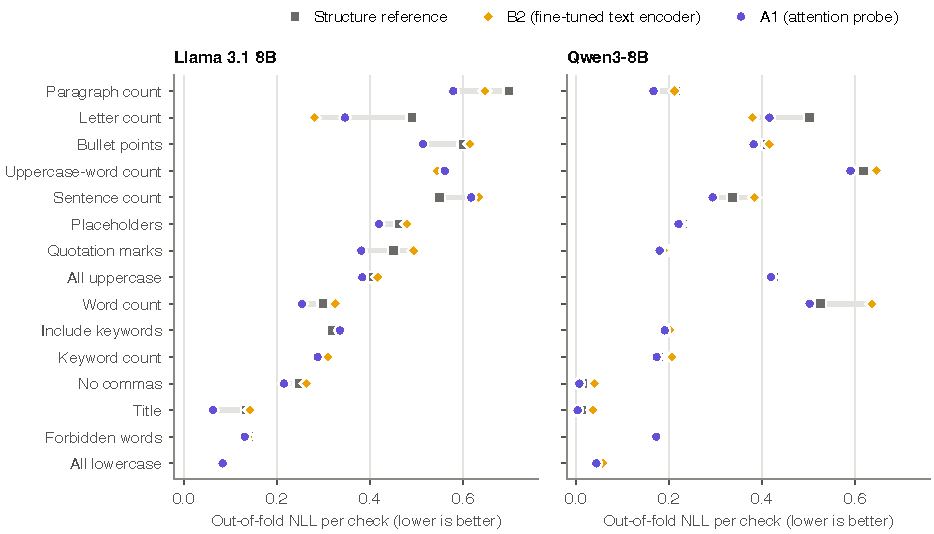
\includegraphics[width=\linewidth]{figures/fig_per_type.pdf}
\caption{Out-of-fold NLL by rule type on the training groups for the structure head, the fine-tuned text baseline B2
and the attention probe A1. Types are ordered by Llama's violation rate. Lower is better.}
\label{fig:pertype}
\end{figure}

\textbf{By rule type.} Figure~\ref{fig:pertype} breaks the Objective~1 loss down by rule type. For Llama, A1 has a
lower loss than B2 on 13 of the 15 types (with an interval excluding zero on 8) and a lower loss than the structure
head on 11 (8). For Qwen the counts are 12 (5) and 14 (5). The largest gains over the structure head for Llama are on
letter count, paragraph count, bullet points, title and quotation marks, which are mostly rules about the layout of
the response. One type goes the other way. For letter count (``the letter \emph{i} should appear less than 9 times''),
B2 has the lowest loss for both generators (0.281 against 0.347 for A1 and 0.491 for the structure head on Llama),
although the interval for its difference from A1 includes zero. The
difficulty of this rule depends on which letter is named, and that information is in the rule text, which the
fine-tuned encoder reads, but not in the structured features. For keyword inclusion, keyword count and all-lowercase, no predictor improves materially on the
type $\times$ $k$ rate.

Within a rule type, discrimination is modest. The mean within-type AUROC over the 15 types is 0.73 for A1 on Llama,
against 0.63 for the structure head and 0.59 for B2. For Qwen the three values are 0.56, 0.54 and 0.58, with three
types violated in fewer than 1\% of checks, where AUROC is unstable (Appendix~\ref{app:pertype}). A large part of the
overall AUROC therefore comes from knowing which rule is being asked about, and the internal features add to it mainly
for Llama.

\textbf{By number of rules.} The advantage of A1 over the structure head grows with $k$. At $k=1$ the two are close
(out-of-fold NLL 0.332 against 0.341 for Llama, 0.154 against 0.155 for Qwen). At $k=5$ the gap is 0.338 against 0.387
for Llama and 0.249 against 0.274 for Qwen (Appendix~\ref{app:oof}). One reading is that with a single rule the rule's type and parameters nearly determine the risk, while with five
rules the outcome depends more on how the model has weighed them against one another, which the internal features
partly reflect. We have not tested this reading.

\subsection{Design choices and component contrasts}

\begin{table}[t]
\centering\small
\caption{Hidden-state probe alone, attention probe alone and both together (cross-validation loss; Objective~2 in units
of $10^{-2}$). The last column is the relative change of the combination against the better of the two single probes.}
\label{tab:comp}
% generated by report/make_tables.py -- do not edit
\begin{tabular}{llcccc}
\toprule
Cell & Hidden probe & Hidden alone & A1 alone & Hidden + A1 & Combined vs better single \\
\midrule
Llama, Obj.~1 & H1 & 0.3761 & 0.3316 & 0.3583 & $+8.1\%$ \\
 & H2 & 0.3390 & 0.3316 & 0.3364 & $+1.5\%$ \\
Llama, Obj.~2 & H1 & 1.656 & 1.693 & 1.585 & $-4.3\%$ \\
 & H2 & 1.643 & 1.693 & 1.603 & $-2.5\%$ \\
Qwen, Obj.~1 & H1 & 0.2613 & 0.2361 & 0.2556 & $+8.3\%$ \\
 & H2 & 0.2396 & 0.2361 & 0.2386 & $+1.1\%$ \\
Qwen, Obj.~2 & H1 & 1.130 & 1.274 & 1.103 & $-2.4\%$ \\
 & H2 & 1.192 & 1.274 & 1.164 & $-2.3\%$ \\
\bottomrule
\end{tabular}

\end{table}

\textbf{Layer and pooling.} The hidden state at 50\% depth is selected in three of the four cells and at 75\% depth for
Objective~2 on Qwen. The last layer is worst in every cell. Summing attention over the rule span is selected over
averaging in every cell, by small margins (Table~\ref{tab:layer}, Appendix~\ref{app:config}).

\textbf{Exact-rule conditioning (RQ4).} In Objective~1, adding the rule embedding to the hidden state (H1 to H2)
lowers the out-of-fold NLL by 0.037 for Llama (0.018 to 0.056) and by 0.021 for Qwen (0.0004 to 0.039). In Objective~2
the interval includes zero for both generators. Per-type heads tell H1 the rule's type but not its parameters or
keywords, and the embedding supplies these.

\textbf{Adding probes to a baseline (RQ3).} In Objective~1, adding any single probe to B1 or to B2 lowers the
out-of-fold NLL for both generators, with every interval excluding zero (families C2 and C3 in
Appendix~\ref{app:contrasts}). This comparison also switches the head from one shared head to per-type heads
(Section~\ref{sec:limits}), so it does not isolate the contribution of the probe features. In Objective~2, where the
head structure does not change, adding H1 or H2 to B1 lowers RMSE for both generators, and adding a probe to B2 makes
no detectable difference.

\textbf{Hidden state plus attention.} Combining the two internal signals does not help per-rule prediction: H1+A1 is
8.1\% (Llama) and 8.3\% (Qwen) worse than A1 alone (Table~\ref{tab:comp}). In Objective~2 the combination is 2.3 to
4.3\% better than the better single probe. One likely cause in Objective~1 is that all blocks share a single penalty
after standardisation, so the 4,096-dimensional hidden state can swamp the roughly 1,000 attention features. We did
not add block-specific penalties, since that would change the specified protocol.

\textbf{Encoder adaptation.} Fine-tuning the text encoder (B1 to B2) lowers the out-of-fold loss for Llama in both
objectives (NLL by 0.017, interval 0.002 to 0.032; RMSE by 0.009, 0.003 to 0.015) and makes no detectable difference
for Qwen.

\subsection{An artefact in the official ``all uppercase'' verifier}
\label{sec:audit}

\begin{table}[t]
\centering\small
\caption{Audit of the ``all uppercase'' rule on the training groups. The official check requires the response to be
upper case and a language detector to return English. ``Language check only'': responses that are entirely upper case
but fail the language step, with their share of all violations of this rule. ``Corrected'': violation rate if those
responses are counted as following the rule.}
\label{tab:ec}
% generated by report/make_tables.py -- do not edit
\begin{tabular}{lcccccccc}
\toprule
 & & & \multicolumn{2}{c}{Cause of violation} & Detected as & Mainly & \multicolumn{2}{c}{Violation rate} \\
\cmidrule(lr){4-5}\cmidrule(lr){8-9}
Generator & Checks & Violations & Not uppercase & Language check only & German & CJK & Official & Corrected \\
\midrule
Llama & 205,200 & 30,467 & 29,186 & 1,281 (4.2\%) & 99.0\% & 0 & 0.148 & 0.142 \\
Qwen & 205,200 & 29,097 & 16,543 & 12,554 (43.1\%) & 92.5\% & 0 & 0.142 & 0.081 \\
\bottomrule
\end{tabular}

\end{table}

The official check for ``your entire response should be in English, and in all capital letters'' requires both that the
text is upper case and that the \texttt{langdetect} library classifies it as English. While reviewing violations by
cause, we found that many responses that are entirely upper case fail only the language step (Table~\ref{tab:ec}). For
Qwen these are 12,554 of 29,097 violations of this rule (43.1\%), or 6.1\% of all its checks of the rule. For Llama they
are 1,281 (4.2\% of violations). The detector labels 92.5\% (Qwen) and 99.0\% (Llama) of them as German. None of the
responses is mainly in a non-Latin script, and when the same text is lower-cased the detector returns English for 9,839
of the 12,554 Qwen responses and 1,263 of the 1,281 Llama responses. Part of the remainder are repetition loops (3,520
of the Qwen responses). The failures concentrate in a few tasks (the ten most affected account for 92\% of Qwen's) and
are far more frequent when the prompt also contains a letter-count rule (16.0\% of Qwen's upper-case responses against
2.2\% otherwise), which pushes the text away from ordinary English letter statistics.

These responses follow the rule as a person would read it. Counting them as followed would lower Qwen's violation rate
on this rule from 14.2\% to 8.1\%. We have not changed any label. The frozen labels use the official verifier, and the
plan already includes a sensitivity analysis that drops this rule type. Section~\ref{sec:next} lists the additional
analysis we are considering.

% ---------------------------------------------------------------------------------------------------------------
\section{Remaining work and goals}
\label{sec:next}

The project has three levels of goals. The first is predictive accuracy: establish, on held-out groups, whether
internal-state probes improve per-rule and per-prompt violation prediction over prompt-only baselines (RQ1 to RQ4). The
second is controlled sensitivity: test whether the predictors anticipate how violation risk changes when one property
of the prompt changes. The third, which is exploratory, is to describe which layers and attention heads carry the
signal. The first two are pre-specified. This section lists what remains, in the order in which it will be done.

\subsection{Decisions before unblinding}

\textbf{Regularisation grid.} The specified grid $\lambda\in\{0.01, 0.1, 1\}$ turned out to be too narrow for some
heads (Table~\ref{tab:l2}, Appendix~\ref{app:config}). The structure head selects the smallest value in all four
cells, and its loss one grid step inwards is 7.9 to 11.1\% higher, so its optimum may lie below the grid. In
Objective~2 several configurations also sit at an edge. This matters for the conclusions, because the structure head is
a key comparator: if a wider grid lowers its loss, the margins in Table~\ref{tab:bestvs} shrink. The option under
consideration is to widen the grid to $\{0.001, 0.01, 0.1, 1, 10\}$ for every configuration, rerun the
cross-validation on training data (about three hours), refit, and freeze the plan again. The alternative is to keep
the grid as specified and report the edge selections as a limitation. Either way the decision is taken, and recorded,
before any test row is read.

\textbf{Verifier-corrected sensitivity analysis.} We are considering adding, to the frozen plan, a sensitivity analysis
that keeps the ``all uppercase'' rule but counts responses that fail only the language step as followed. It would use
derived labels and leave the primary labels untouched.

\subsection{Confirmatory evaluation on the held-out groups}

After unblinding is recorded, each refitted model is applied once to the 15 test groups (11,070 prompts and 46,170
prompt--rule rows per generator).

\textbf{Metrics.} Objective~1: NLL per check (primary), Brier score, expected calibration error, AUROC, and the observed
violation rate in the top and bottom deciles of predicted risk, overall, per rule type and per $k$. Objective~2: RMSE
(primary), mean absolute error, calibration error, and Pearson and Spearman correlation. Calibration bins are fixed in
advance from each configuration's out-of-fold training predictions.

\textbf{Uncertainty.} A paired cluster bootstrap over the 15 test groups \citep{efron1979bootstrap}, with 10,000
replicates and the same replicate weights for every configuration, gives 95\% percentile intervals for every metric
and difference.

\textbf{Contrasts.} Table~\ref{tab:contrasts} lists the 37 pre-specified contrasts, run for each generator and
objective on the primary metric. Each has a two-sided bootstrap $p$-value, adjusted by Holm's method
\citep{holm1979} within each family, generator and objective. Per-type and per-$k$ breakdowns are descriptive.

\begin{table}[t]
\centering\small
\caption{Pre-specified contrast families for the test evaluation. Each contrast compares two configurations on the
primary metric. ``Better of'' is decided by training cross-validation loss.}
\label{tab:contrasts}
\begin{tabular}{llp{6.1cm}l}
\toprule
Family & Question & Contrasts & Number \\
\midrule
C1 & Internal state vs prompt-only & B1 and B2 against each of H1, H2, A1 & 6 \\
C2 & Hidden-state increment & B1 vs B1+H1, B1+H2; B2 vs B2+H1, B2+H2 & 4 \\
C3 & Attention increment & B1 vs B1+A1; B2 vs B2+A1 & 2 \\
C4 & Complementarity & Better of (H, A1) vs H+A1; baseline+H vs baseline+H+A1; baseline+A1 vs baseline+H+A1 & 10 \\
C5 & Exact-rule conditioning & H1 vs H2, alone and with B1, B2 or A1 & 4 \\
C6 & Encoder adaptation & B1 vs B2, alone and with H1, H2 or A1 & 4 \\
Ref. & Probe vs known structure & Structure head against each probe-only configuration & 7 \\
\bottomrule
\end{tabular}
\end{table}

\textbf{What would count as an answer.} For RQ1 and RQ2, support requires C1 contrasts against B2, the more demanding baseline, that favour the probe on the test groups
with Holm-adjusted $p<0.05$, together with the corresponding structure-head contrasts. The training results lead us to expect this for A1 and H2 in Objective~1 and for H1 in Objective~2 on Qwen,
and not for Objective~2 on Llama. For RQ3, the C2 and C3 contrasts test whether adding a probe to a baseline helps. For
RQ4, C5. A result in which the probes do not beat B2 on held-out groups would be reported as such: the claim under test
is incremental predictive value, not that internal states contain information absent from the prompt.

\subsection{Controlled analyses}

The balanced design supports matched comparisons in which one property changes and the rest is held fixed. For each
pair of prompts we compare the change a predictor forecasts with the change observed in the labels, scoring the mean
absolute error of the predicted change and, on pairs whose observed difference is reliably non-zero (a 95\% interval that excludes zero: Agresti--Caffo for
Objective~1 \citep{agresti2000}, Welch for Objective~2), whether the predicted direction is right. The pairs are defined from the design alone, so they are
fixed before the test set is read (Table~\ref{tab:pairs}).
\begin{itemize}
\item \textbf{A, position.} Same task, rule set and target rule; the target rule moves to another position.
\item \textbf{B, count.} Same task and chain; one rule is appended ($k$ to $k+1$).
\item \textbf{C, composition.} Same task, $k$, target rule and position; exactly one accompanying rule is swapped.
\item \textbf{D, task.} Identical ordered rule list on two different tasks of the group.
\item \textbf{E, difficulty.} Test metrics by tercile of rule-type difficulty, with terciles fixed from training rates
at $k=1$.
\end{itemize}

\begin{table}[t]
\centering\small
\caption{Matched pairs available on the 15 test groups for the controlled analyses (fixed by the design).}
\label{tab:pairs}
\begin{tabular}{lrrrr}
\toprule
 & A, position & B, count & C, composition & D, task \\
\midrule
Objective~1 (rule-level pairs) & 22,950 & 2,700 & 25,380 & 46,170 \\
Objective~2 (prompt-level pairs) & -- & 1,080 & 7,560 & 11,070 \\
\bottomrule
\end{tabular}
\end{table}

\subsection{Sensitivity analyses and exploratory extensions}

\textbf{Pre-specified sensitivity analyses.} The primary test metrics will be recomputed with labels that exclude
truncated responses, without the ``all uppercase'' rule type, and without prompts that have any response in a
repetition loop.

\textbf{Exploratory extensions.} These are not pre-specified and will be labelled as exploratory wherever they are
reported. (i)~Which layers and heads carry the attention signal, and whether a small subset suffices. (ii)~Whether
block-specific regularisation makes hidden-state and attention features complementary in Objective~1. (iii)~A control
for head structure: in Objective~1, adding a probe to B1 or B2 also changes one shared head into 15 per-type heads, so
giving the baselines per-type heads would separate the two effects. (iv)~Transfer of a predictor trained on one
generator to the other.

\textbf{Deliverables.} The final report will add the test results, contrasts and controlled analyses to the sections
that are marked pending here, with every number generated from saved tables, and we intend to release the manifest,
labels and analysis code.

% ---------------------------------------------------------------------------------------------------------------
\section{Limitations}
\label{sec:limits}

\textbf{No held-out results yet.} Every number in Section~\ref{sec:results} is from training groups. Cross-validation
losses of selected settings are slightly optimistic, and the out-of-fold intervals describe variation across training
groups only.

\textbf{Regularisation grid.} Several heads select an edge of the $\lambda$ grid, including the structure head in every
cell (Section~\ref{sec:next}). The comparators may be under-tuned relative to what a wider grid would give.

\textbf{Fewer distinct comparisons than names.} Only 15 of the 23 configurations have distinct inputs, so some
pre-specified contrasts compare identical feature sets. They are kept in the Holm families, which makes the adjustment
slightly conservative.

\textbf{Head structure is confounded with probe features in Objective~1.} Baselines alone use one shared head, and
baseline-plus-probe configurations use per-type heads. The C2 and C3 contrasts therefore measure both changes together.

\textbf{Feature fusion.} All blocks share one penalty. The finding that H1+A1 is worse than A1 alone in Objective~1 may
reflect this choice, not an absence of complementary information.

\textbf{Label noise.} With 20 samples, $\phat$ has a standard error of up to 0.11. The official verifiers are imperfect
(Section~\ref{sec:audit}), and for Qwen 2.5\% of responses hit the token limit and 2.1\% contain repetition loops
(0.2\% and 0.1\% for Llama).

\textbf{Sparse rule types.} Some types are almost never violated by one generator (Qwen and the title rule), so their
per-type heads are fitted on very few violated responses.

\textbf{Scope.} Two open 8B models, English prompts, 15 programmatically verifiable rule types, at most five rules per
prompt, and default decoding settings. The test set shares rule types, and many exact rules, with the training set.
With 15 test groups, power to detect small differences is limited. The task-family labels are ours.

\textbf{Backends.} Internal features were computed on a different backend from the one that generated the responses.
They approximate the generating states (cosine at least 0.998 in the pilot) but are not identical to them.

\textbf{Interpretation.} A probe that predicts violations shows that the information is linearly or near-linearly
available in the features. It does not show that the model uses those features, or that attention patterns cause
violations.

% ---------------------------------------------------------------------------------------------------------------
\section{Conclusion}

We built a controlled multi-instruction dataset with repeated sampling and a pre-specified protocol for asking whether
a model's internal state at the end of the prompt predicts rule violations beyond what the prompt reveals. On the
training groups, the answer so far is a qualified yes. Attention from the final prompt token to a rule's span is the
best single predictor of whether that rule will be violated, for both generators, and it improves on a text encoder
fine-tuned for the same task. The improvement concentrates on layout and length rules and grows with the number of
rules in the prompt. It is not universal. A hidden-state probe that is not told the exact rule does no better than
structured prompt features, the fine-tuned text encoder wins where the difficulty lies in the rule's wording, and for
one generator it matches the probes on per-prompt prediction. Whether these patterns hold on unseen tasks and rule
combinations is the subject of the confirmatory evaluation, which has not yet been run.

\subsection*{Reproducibility statement}
The ManyIFEval commit, model revisions, chat templates, decoding settings, random seeds and package versions are pinned
and recorded. Generation, verification and feature extraction are resumable and write hashed manifests. Every table in this draft is generated from saved result files by a script, and the numbers quoted in the text are
checked against those files automatically. The analysis
plan is stored with a SHA-256 hash, alongside hashes of the folds, the manifest and the source tree. One wording-only
edit to the report generator was made a minute after the freeze, so the recorded source-tree hash differs from the
current one by that edit; the hash of the analysis plan is unchanged.

\subsection*{Ethics statement}
The study uses public benchmark prompts and openly released models, and involves no human subjects or personal data.
Predicting instruction violations is intended to make model behaviour more predictable. We see no specific risk of
misuse.

\subsection*{Use of AI tools}
An AI coding assistant was used, under the authors' direction, to implement the pipeline, run the analyses and draft
this report. The authors reviewed the work and are responsible for its content.

\bibliographystyle{plainnat}
\bibliography{refs}

% ===============================================================================================================
\clearpage
\appendix

\section{Rule types and an example prompt}
\label{app:types}

\begin{table}[H]
\centering\footnotesize
\caption{The 15 rule types: category, the parameters drawn by the released code's default generators (``relation'' is
``less than'' or ``at least''), the number of training and test groups whose pool contains the type, and the violation
rate on the training groups with a 95\% interval.}
\label{tab:types}
\setlength{\tabcolsep}{4pt}
% generated by report/make_tables.py -- do not edit
\begin{tabular}{lllccc}
\toprule
Rule type & Category & Sampled parameters & Groups (train / test) & Llama violation rate & Qwen violation rate \\
\midrule
Paragraph count & length/counts & $N\in[1,5]$ & 21 / 4 & $0.511$ {\scriptsize[$0.410$, $0.605$]} & $0.059$ {\scriptsize[$0.018$, $0.105$]} \\
Letter count & length/counts & letter, $N\in[1,10]$, relation & 32 / 9 & $0.365$ {\scriptsize[$0.216$, $0.513$]} & $0.341$ {\scriptsize[$0.194$, $0.488$]} \\
Bullet points & formatting & $N\in[1,5]$ & 28 / 8 & $0.292$ {\scriptsize[$0.237$, $0.345$]} & $0.144$ {\scriptsize[$0.108$, $0.183$]} \\
Uppercase-word count & letter case & $N\in[1,20]$, relation & 15 / 3 & $0.249$ {\scriptsize[$0.134$, $0.373$]} & $0.255$ {\scriptsize[$0.171$, $0.359$]} \\
Sentence count & length/counts & $N\in[1,20]$, relation & 14 / 4 & $0.226$ {\scriptsize[$0.134$, $0.322$]} & $0.128$ {\scriptsize[$0.043$, $0.235$]} \\
Placeholders & formatting & $N\in[1,4]$ & 29 / 8 & $0.202$ {\scriptsize[$0.145$, $0.266$]} & $0.063$ {\scriptsize[$0.035$, $0.097$]} \\
Quotation marks & start/end & none & 26 / 6 & $0.192$ {\scriptsize[$0.130$, $0.262$]} & $0.046$ {\scriptsize[$0.019$, $0.085$]} \\
All uppercase & letter case & none & 20 / 6 & $0.148$ {\scriptsize[$0.115$, $0.187$]} & $0.142$ {\scriptsize[$0.097$, $0.195$]} \\
Word count & length/counts & $N\in[100,500]$, relation & 16 / 4 & $0.104$ {\scriptsize[$0.039$, $0.180$]} & $0.210$ {\scriptsize[$0.108$, $0.316$]} \\
Include keywords & keywords & 2 words & 16 / 6 & $0.098$ {\scriptsize[$0.065$, $0.131$]} & $0.047$ {\scriptsize[$0.025$, $0.073$]} \\
Keyword count & keywords & 1 word, $N\in[1,3]$, relation & 20 / 6 & $0.077$ {\scriptsize[$0.038$, $0.121$]} & $0.040$ {\scriptsize[$0.017$, $0.068$]} \\
No commas & punctuation & none & 30 / 8 & $0.077$ {\scriptsize[$0.051$, $0.105$]} & $0.001$ {\scriptsize[$0.000$, $0.002$]} \\
Title & formatting & none & 31 / 6 & $0.031$ {\scriptsize[$0.012$, $0.057$]} & $0.000$ {\scriptsize[$0.000$, $0.001$]} \\
Forbidden words & keywords & 2 words & 31 / 9 & $0.029$ {\scriptsize[$0.013$, $0.049$]} & $0.036$ {\scriptsize[$0.016$, $0.062$]} \\
All lowercase & letter case & none & 13 / 3 & $0.016$ {\scriptsize[$0.007$, $0.029$]} & $0.007$ {\scriptsize[$0.003$, $0.013$]} \\
\bottomrule
\end{tabular}

\end{table}

An example prompt with $k=3$:
\begin{quote}\footnotesize\ttfamily
Write a resume for a fresh high school graduate who is seeking their first job.\\[3pt]
Your response should follow the instructions below:\\
- There should be 3 paragraphs. Paragraphs are separated with the markdown divider: ***\\
- Your answer must contain a title, wrapped in double angular brackets, such as <<poem of joy>>.\\
- In your response, the letter i should appear less than 9 times.
\end{quote}

\section{Descriptive statistics}
\label{app:desc}

\begin{figure}[H]
\centering
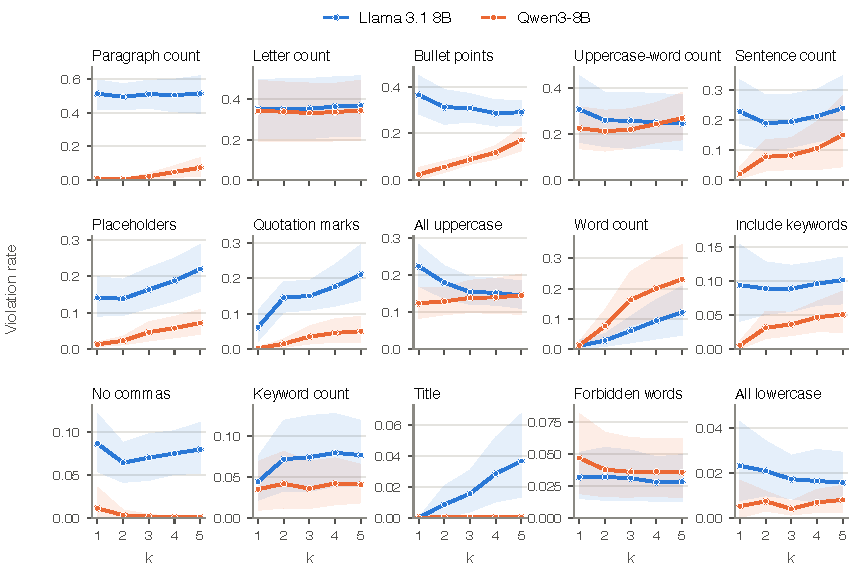
\includegraphics[width=\linewidth]{figures/fig_type_by_k.pdf}
\caption{Violation rate by rule type and number of rules on the training groups, with 95\% bands. Vertical scales
differ between panels.}
\label{fig:typek}
\end{figure}

\begin{table}[H]
\centering\small
\caption{Label distribution and response quality on the training groups. $v$: number of the 20 responses that violate
the rule. Truncated: the response reached the 2,048-token limit.}
\label{tab:quality}
% generated by report/make_tables.py -- do not edit
\begin{tabular}{lccccccc}
\toprule
 & \multicolumn{3}{c}{Prompt--rule rows ($\hat p$)} & \multicolumn{2}{c}{Prompts ($\hat q$)} & \multicolumn{2}{c}{Responses} \\
\cmidrule(lr){2-4}\cmidrule(lr){5-6}\cmidrule(lr){7-8}
Generator & $v=0$ & $v=20$ & Mean & Median & $\hat q=0$ & Truncated & Repetition loop \\
\midrule
Llama & 53.2\% & 5.4\% & 0.177 & 0.150 & 10.4\% & 0.18\% & 0.08\% \\
Qwen & 74.6\% & 3.9\% & 0.099 & 0.033 & 34.3\% & 2.49\% & 2.05\% \\
\bottomrule
\end{tabular}

\end{table}

\section{Configuration details}
\label{app:config}

\textbf{Structured features.} \blk{S1} (75 columns): $k$ and its one-hot encoding (6); target type one-hot (15);
position, relative position, first and last indicators (4); the target's numeric parameter and relation (13); which
other types are present (15); their parameters, summed (13); task family (6); prompt length in tokens and characters
and task length (3). \blk{S2} (175 columns) holds the same information for all five rule slots. Keywords and the letter
of a letter-count rule are not in the structured features. They reach a predictor only through a rule-text embedding.

\textbf{Identical feature sets.} With one shared hidden-state layer and duplicate blocks removed, the following have
the same inputs in both objectives: H2 and H1+H2; H2+A1 and H1+H2+A1; B1+H1, B1+H2 and B1+H1+H2; B1+H1+A1, B1+H2+A1
and B1+H1+H2+A1; B2+H2 and B2+H1+H2; B2+H2+A1 and B2+H1+H2+A1.

\textbf{Training details.} Linear heads: full-batch L-BFGS, up to 500 iterations. MLP heads: Adam, learning rate
$10^{-3}$, batches of 1,024 rows, up to 30 epochs. The penalty is $(\lambda/2)\lVert W\rVert^2$ on weight matrices,
added to the mean loss. B2: LoRA rank 16, $\alpha=32$, dropout 0.05 on the query, key, value and dense layers; AdamW,
batches of 32 prompts, weight decay 0.01, 5\% warm-up and linear decay. Head selection took about 4.4 hours (Objective~1)
and 2.2 hours (Objective~2) per generator on a laptop CPU, and the B2 grid about 6 GPU-hours.

\begin{table}[H]
\centering\small
\caption{Selection of the hidden-state layer (on H1) and of the attention pooling (on A1) by cross-validation loss.
Objective~2 in units of $10^{-2}$. Bold: selected.}
\label{tab:layer}
% generated by report/make_tables.py -- do not edit
\begin{tabular}{lccccc}
\toprule
 & \multicolumn{3}{c}{H1 by hidden-state depth} & \multicolumn{2}{c}{A1 by span pooling} \\
\cmidrule(lr){2-4}\cmidrule(lr){5-6}
Cell & 50\% & 75\% & 100\% & Sum & Mean \\
\midrule
Llama, Obj.~1 & \textbf{0.3761} & 0.3973 & 0.3982 & \textbf{0.3316} & 0.3332 \\
Llama, Obj.~2 & \textbf{1.656} & 1.872 & 1.889 & \textbf{1.693} & 1.737 \\
Qwen, Obj.~1 & \textbf{0.2613} & 0.2650 & 0.2742 & \textbf{0.2361} & 0.2367 \\
Qwen, Obj.~2 & 1.186 & \textbf{1.130} & 1.269 & \textbf{1.274} & 1.284 \\
\bottomrule
\end{tabular}

\end{table}

\begin{table}[H]
\centering\small
\caption{B2 fine-tuning grid: cross-validation loss of the jointly trained head, used only to select the learning rate
and number of epochs (Objective~2 in units of $10^{-2}$). Bold: selected.}
\label{tab:b2}
% generated by report/make_tables.py -- do not edit
\begin{tabular}{lcccc}
\toprule
 & \multicolumn{2}{c}{LR $1\times10^{-4}$} & \multicolumn{2}{c}{LR $2\times10^{-4}$} \\
\cmidrule(lr){2-3}\cmidrule(lr){4-5}
Cell & 1 epoch & 3 epochs & 1 epoch & 3 epochs \\
\midrule
Llama, Obj.~1 & \textbf{0.3724} & 0.3784 & 0.3771 & 0.3820 \\
Llama, Obj.~2 & 1.926 & 1.703 & 1.787 & \textbf{1.647} \\
Qwen, Obj.~1 & \textbf{0.2687} & 0.2980 & 0.2772 & 0.2923 \\
Qwen, Obj.~2 & 1.547 & 1.437 & \textbf{1.433} & 1.529 \\
\bottomrule
\end{tabular}

\end{table}

\begin{table}[H]
\centering\small
\caption{Selected penalty strength $\lambda$ across the 23 configurations and the structure head, and what the loss
would be one grid step inwards for heads that selected an edge value.}
\label{tab:l2}
% generated by report/make_tables.py -- do not edit
\begin{tabular}{lcccccc}
\toprule
 & \multicolumn{3}{c}{Selected $\lambda$ (24 heads)} & Configurations at an edge & \multicolumn{2}{c}{Loss increase one step inwards} \\
\cmidrule(lr){2-4}\cmidrule(lr){6-7}
Cell & 0.01 & 0.1 & 1 & (lowest / highest) & Structure head & Largest, configurations \\
\midrule
Llama, Obj.~1 & 2 & 22 & 0 & 1 / 0 & 7.9\% & 2.9\% \\
Llama, Obj.~2 & 8 & 9 & 7 & 7 / 7 & 8.6\% & 23.4\% \\
Qwen, Obj.~1 & 1 & 18 & 5 & 0 / 5 & 9.2\% & 3.9\% \\
Qwen, Obj.~2 & 6 & 18 & 0 & 5 / 0 & 11.1\% & 21.6\% \\
\bottomrule
\end{tabular}

\end{table}

\clearpage
\section{Cross-validation results for all configurations}
\label{app:fullcv}

\begin{table}[H]
\centering\scriptsize
\caption{Llama 3.1 8B: selected head, cross-validation loss and standard deviation over the five folds for the four
references and all 23 configurations. Width: number of input features. Head: linear (lin) or MLP, penalty $\lambda$,
and the selected number of epochs for MLPs. The fold standard deviation mostly reflects folds that are harder for every
configuration, so it overstates the uncertainty of differences between rows.}
\setlength{\tabcolsep}{4pt}
% generated by report/make_tables.py -- do not edit
\begin{tabular}{lrlccrlcc}
\toprule
 & \multicolumn{4}{c}{Objective 1 (NLL)} & \multicolumn{4}{c}{Objective 2 (MSE $\times 10^{-2}$)} \\
\cmidrule(lr){2-5}\cmidrule(lr){6-9}
Configuration & Width & Head, $\lambda$/epoch & CV loss & Fold SD & Width & Head, $\lambda$/epoch & CV loss & Fold SD \\
\midrule
Constant rate & -- & rates & 0.4705 & 0.0586 & -- & rates & 2.364 & 0.068 \\
Type rate & -- & rates & 0.4155 & 0.0430 & -- & rates & 2.046 & 0.108 \\
Type $\times$ $k$ rate & -- & rates & 0.4152 & 0.0428 & -- & rates & 2.036 & 0.102 \\
Structure head & 75 & MLP, 0.01/10 & 0.3779 & 0.0409 & 175 & lin, 0.01 & 1.847 & 0.199 \\
\midrule
H1 & 4,096 & MLP, 0.1/23 & 0.3761 & 0.0300 & 4,197 & lin, 0.01 & 1.656 & 0.223 \\
H2 & 5,120 & MLP, 0.1/6 & 0.3390 & 0.0326 & 9,317 & lin, 0.1 & 1.643 & 0.199 \\
A1 & 1,024 & MLP, 0.01/9 & 0.3316 & 0.0263 & 5,131 & lin, 0.01 & 1.693 & 0.193 \\
H1+H2 & 5,120 & MLP, 0.1/11 & 0.3396 & 0.0348 & 9,317 & lin, 0.1 & 1.643 & 0.199 \\
H1+A1 & 5,120 & MLP, 0.1/7 & 0.3583 & 0.0361 & 9,322 & lin, 0.01 & 1.585 & 0.222 \\
H2+A1 & 6,144 & MLP, 0.1/7 & 0.3364 & 0.0318 & 14,442 & lin, 0.1 & 1.603 & 0.207 \\
H1+H2+A1 & 6,144 & MLP, 0.1/7 & 0.3363 & 0.0347 & 14,442 & lin, 0.1 & 1.603 & 0.207 \\
\midrule
B1 & 2,123 & MLP, 0.1/4 & 0.3868 & 0.0432 & 6,319 & MLP, 0.01/23 & 1.838 & 0.171 \\
B1+H1 & 6,219 & MLP, 0.1/8 & 0.3429 & 0.0292 & 10,415 & MLP, 0.01/25 & 1.642 & 0.194 \\
B1+H2 & 6,219 & MLP, 0.1/8 & 0.3415 & 0.0332 & 10,415 & MLP, 0.01/18 & 1.669 & 0.160 \\
B1+A1 & 3,147 & MLP, 0.1/5 & 0.3451 & 0.0313 & 11,444 & lin, 0.1 & 1.774 & 0.213 \\
B1+H1+H2 & 6,219 & MLP, 0.1/6 & 0.3393 & 0.0350 & 10,415 & MLP, 0.01/26 & 1.691 & 0.207 \\
B1+H1+A1 & 7,243 & MLP, 0.1/6 & 0.3390 & 0.0290 & 15,540 & lin, 0.1 & 1.638 & 0.207 \\
B1+H2+A1 & 7,243 & MLP, 0.1/19 & 0.3410 & 0.0267 & 15,540 & lin, 0.1 & 1.638 & 0.207 \\
B1+H1+H2+A1 & 7,243 & MLP, 0.1/6 & 0.3407 & 0.0348 & 15,540 & lin, 0.1 & 1.638 & 0.207 \\
\midrule
B2 & 2,123 & MLP, 0.1/1 & 0.3700 & 0.0389 & 6,319 & MLP, 0.1/1 & 1.613 & 0.150 \\
B2+H1 & 6,219 & MLP, 0.1/3 & 0.3365 & 0.0284 & 10,415 & lin, 1 & 1.583 & 0.235 \\
B2+H2 & 7,243 & MLP, 0.1/5 & 0.3347 & 0.0293 & 15,535 & lin, 1 & 1.565 & 0.231 \\
B2+A1 & 3,147 & MLP, 0.1/3 & 0.3472 & 0.0337 & 11,444 & lin, 1 & 1.594 & 0.229 \\
B2+H1+H2 & 7,243 & MLP, 0.1/11 & 0.3345 & 0.0304 & 15,535 & lin, 1 & 1.565 & 0.231 \\
B2+H1+A1 & 7,243 & MLP, 0.1/19 & 0.3350 & 0.0285 & 15,540 & lin, 1 & 1.573 & 0.236 \\
B2+H2+A1 & 8,267 & MLP, 0.1/16 & 0.3353 & 0.0284 & 20,660 & lin, 1 & 1.562 & 0.233 \\
B2+H1+H2+A1 & 8,267 & MLP, 0.1/10 & 0.3341 & 0.0254 & 20,660 & lin, 1 & 1.562 & 0.233 \\
\bottomrule
\end{tabular}

\end{table}

\begin{table}[H]
\centering\scriptsize
\caption{Qwen3-8B: as the previous table.}
\setlength{\tabcolsep}{4pt}
% generated by report/make_tables.py -- do not edit
\begin{tabular}{lrlccrlcc}
\toprule
 & \multicolumn{4}{c}{Objective 1 (NLL)} & \multicolumn{4}{c}{Objective 2 (MSE $\times 10^{-2}$)} \\
\cmidrule(lr){2-5}\cmidrule(lr){6-9}
Configuration & Width & Head, $\lambda$/epoch & CV loss & Fold SD & Width & Head, $\lambda$/epoch & CV loss & Fold SD \\
\midrule
Constant rate & -- & rates & 0.3256 & 0.0486 & -- & rates & 1.577 & 0.235 \\
Type rate & -- & rates & 0.2765 & 0.0369 & -- & rates & 1.379 & 0.163 \\
Type $\times$ $k$ rate & -- & rates & 0.2756 & 0.0365 & -- & rates & 1.350 & 0.156 \\
Structure head & 75 & MLP, 0.01/3 & 0.2573 & 0.0435 & 175 & lin, 0.01 & 1.275 & 0.231 \\
\midrule
H1 & 4,096 & MLP, 1/2 & 0.2613 & 0.0371 & 4,197 & lin, 0.01 & 1.130 & 0.178 \\
H2 & 5,120 & MLP, 0.1/21 & 0.2396 & 0.0367 & 9,317 & lin, 0.1 & 1.192 & 0.077 \\
A1 & 1,152 & MLP, 0.1/8 & 0.2361 & 0.0308 & 5,771 & lin, 0.01 & 1.274 & 0.093 \\
H1+H2 & 5,120 & MLP, 0.1/15 & 0.2403 & 0.0398 & 9,317 & lin, 0.1 & 1.192 & 0.077 \\
H1+A1 & 5,248 & MLP, 0.1/24 & 0.2556 & 0.0310 & 9,962 & lin, 0.01 & 1.103 & 0.170 \\
H2+A1 & 6,272 & MLP, 0.1/12 & 0.2386 & 0.0393 & 15,082 & lin, 0.1 & 1.164 & 0.075 \\
H1+H2+A1 & 6,272 & MLP, 0.1/5 & 0.2358 & 0.0367 & 15,082 & lin, 0.1 & 1.164 & 0.075 \\
\midrule
B1 & 2,123 & MLP, 0.1/2 & 0.2646 & 0.0297 & 6,319 & MLP, 0.01/16 & 1.360 & 0.148 \\
B1+H1 & 6,219 & MLP, 0.1/5 & 0.2396 & 0.0369 & 10,415 & lin, 0.1 & 1.224 & 0.092 \\
B1+H2 & 6,219 & MLP, 0.1/11 & 0.2401 & 0.0303 & 10,415 & lin, 0.1 & 1.224 & 0.092 \\
B1+A1 & 3,275 & MLP, 0.1/17 & 0.2379 & 0.0334 & 12,084 & lin, 0.1 & 1.323 & 0.087 \\
B1+H1+H2 & 6,219 & MLP, 0.1/4 & 0.2395 & 0.0370 & 10,415 & MLP, 0.01/25 & 1.209 & 0.061 \\
B1+H1+A1 & 7,371 & MLP, 0.1/12 & 0.2387 & 0.0330 & 16,180 & lin, 0.1 & 1.199 & 0.086 \\
B1+H2+A1 & 7,371 & MLP, 0.1/26 & 0.2387 & 0.0356 & 16,180 & lin, 0.1 & 1.199 & 0.086 \\
B1+H1+H2+A1 & 7,371 & MLP, 0.1/21 & 0.2374 & 0.0310 & 16,180 & lin, 0.1 & 1.199 & 0.086 \\
\midrule
B2 & 2,123 & MLP, 1/21 & 0.2606 & 0.0303 & 6,319 & MLP, 0.1/28 & 1.379 & 0.170 \\
B2+H1 & 6,219 & MLP, 0.1/17 & 0.2359 & 0.0403 & 10,415 & MLP, 0.1/5 & 1.375 & 0.174 \\
B2+H2 & 7,243 & MLP, 1/2 & 0.2349 & 0.0343 & 15,535 & MLP, 0.1/30 & 1.348 & 0.139 \\
B2+A1 & 3,275 & MLP, 1/2 & 0.2409 & 0.0355 & 12,084 & MLP, 0.1/30 & 1.365 & 0.191 \\
B2+H1+H2 & 7,243 & MLP, 0.1/23 & 0.2331 & 0.0406 & 15,535 & MLP, 0.1/22 & 1.357 & 0.164 \\
B2+H1+A1 & 7,371 & MLP, 1/2 & 0.2358 & 0.0358 & 16,180 & MLP, 0.1/17 & 1.365 & 0.175 \\
B2+H2+A1 & 8,395 & MLP, 0.1/17 & 0.2348 & 0.0431 & 21,300 & MLP, 0.1/15 & 1.342 & 0.130 \\
B2+H1+H2+A1 & 8,395 & MLP, 0.1/28 & 0.2324 & 0.0387 & 21,300 & MLP, 0.1/4 & 1.357 & 0.149 \\
\bottomrule
\end{tabular}

\end{table}

\clearpage
\section{Out-of-fold metrics and breakdowns}
\label{app:oof}

\begin{table}[H]
\centering\small
\caption{Out-of-fold metrics on the training groups, Objective~2. The interval is for RMSE.}
\label{tab:oof2}
% generated by report/make_tables.py -- do not edit
\begin{tabular}{llccccc}
\toprule
 & Predictor & RMSE & 95\% interval & MAE & Pearson & Spearman \\
\midrule
Llama & Type $\times$ $k$ rate & 0.1428 & {\scriptsize[0.1343, 0.1518]} & 0.1130 & 0.336 & 0.329 \\
 & Structure head & 0.1360 & {\scriptsize[0.1276, 0.1456]} & 0.1075 & 0.440 & 0.470 \\
 & B1 & 0.1356 & {\scriptsize[0.1272, 0.1437]} & 0.1067 & 0.447 & 0.453 \\
 & B2 & 0.1269 & {\scriptsize[0.1190, 0.1352]} & 0.0986 & 0.543 & 0.537 \\
 & H1 & 0.1285 & {\scriptsize[0.1203, 0.1365]} & 0.1008 & 0.541 & 0.533 \\
 & H2 & 0.1281 & {\scriptsize[0.1199, 0.1360]} & 0.1015 & 0.533 & 0.537 \\
 & A1 & 0.1299 & {\scriptsize[0.1218, 0.1381]} & 0.1026 & 0.513 & 0.493 \\
 & H1+A1\,{\scriptsize(best probe-only)} & 0.1257 & {\scriptsize[0.1173, 0.1340]} & 0.0982 & 0.568 & 0.551 \\
 & B2+H2+A1\,{\scriptsize(lowest CV loss)} & 0.1248 & {\scriptsize[0.1157, 0.1342]} & 0.0940 & 0.575 & 0.561 \\
\midrule
Qwen & Type $\times$ $k$ rate & 0.1160 & {\scriptsize[0.1066, 0.1257]} & 0.0898 & 0.363 & 0.372 \\
 & Structure head & 0.1128 & {\scriptsize[0.1018, 0.1245]} & 0.0866 & 0.425 & 0.419 \\
 & B1 & 0.1164 & {\scriptsize[0.1058, 0.1274]} & 0.0898 & 0.358 & 0.355 \\
 & B2 & 0.1173 & {\scriptsize[0.1057, 0.1308]} & 0.0919 & 0.344 & 0.287 \\
 & H1 & 0.1062 & {\scriptsize[0.0975, 0.1155]} & 0.0803 & 0.521 & 0.481 \\
 & H2 & 0.1091 & {\scriptsize[0.0997, 0.1195]} & 0.0848 & 0.483 & 0.457 \\
 & A1 & 0.1130 & {\scriptsize[0.1029, 0.1240]} & 0.0862 & 0.428 & 0.427 \\
 & H1+A1\,{\scriptsize(best probe-only; lowest CV loss)} & 0.1050 & {\scriptsize[0.0960, 0.1148]} & 0.0785 & 0.537 & 0.501 \\
\bottomrule
\end{tabular}

\end{table}

\begin{figure}[H]
\centering
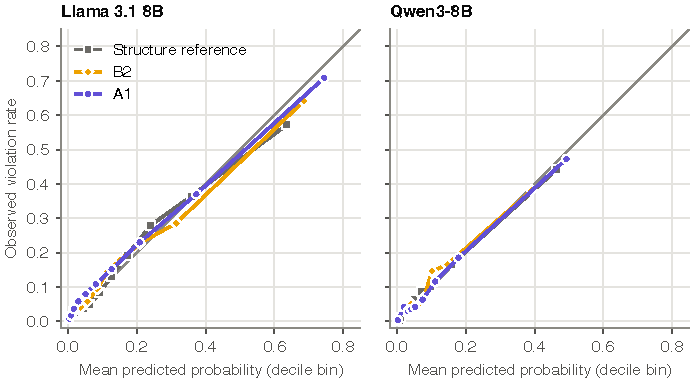
\includegraphics[width=0.78\linewidth]{figures/fig_reliability.pdf}
\caption{Reliability of out-of-fold Objective~1 predictions on the training groups, in decile bins of the predicted
probability.}
\label{fig:reliability}
\end{figure}

\begin{table}[H]
\centering\small
\caption{Out-of-fold primary metric by number of rules on the training groups.}
\label{tab:perk}
% generated by report/make_tables.py -- do not edit
\begin{tabular}{llccccc}
\toprule
Cell & Predictor & $k=1$ & $k=2$ & $k=3$ & $k=4$ & $k=5$ \\
\midrule
Llama, Obj.~1 (NLL) & Structure head & 0.3409 & 0.3447 & 0.3555 & 0.3700 & 0.3870 \\
 & B1 & 0.3597 & 0.3581 & 0.3648 & 0.3798 & 0.3953 \\
 & B2 & 0.3618 & 0.3498 & 0.3527 & 0.3640 & 0.3768 \\
 & H1 & 0.3411 & 0.3409 & 0.3538 & 0.3679 & 0.3848 \\
 & H2 & 0.3190 & 0.3166 & 0.3237 & 0.3316 & 0.3455 \\
 & A1 & 0.3320 & 0.3124 & 0.3159 & 0.3236 & 0.3384 \\
\midrule
Llama, Obj.~2 (RMSE) & Structure head & 0.2753 & 0.1799 & 0.1470 & 0.1288 & 0.1202 \\
 & B1 & 0.2602 & 0.1747 & 0.1474 & 0.1297 & 0.1209 \\
 & B2 & 0.2451 & 0.1683 & 0.1395 & 0.1215 & 0.1118 \\
 & H1 & 0.2359 & 0.1665 & 0.1383 & 0.1236 & 0.1156 \\
 & H2 & 0.2529 & 0.1687 & 0.1382 & 0.1219 & 0.1138 \\
 & A1 & 0.2346 & 0.1687 & 0.1420 & 0.1246 & 0.1168 \\
\midrule
Qwen, Obj.~1 (NLL) & Structure head & 0.1549 & 0.1872 & 0.2202 & 0.2450 & 0.2736 \\
 & B1 & 0.1758 & 0.2016 & 0.2293 & 0.2535 & 0.2787 \\
 & B2 & 0.1704 & 0.1965 & 0.2245 & 0.2487 & 0.2754 \\
 & H1 & 0.1691 & 0.1965 & 0.2272 & 0.2498 & 0.2759 \\
 & H2 & 0.1636 & 0.1886 & 0.2161 & 0.2315 & 0.2515 \\
 & A1 & 0.1540 & 0.1767 & 0.2070 & 0.2275 & 0.2485 \\
\midrule
Qwen, Obj.~2 (RMSE) & Structure head & 0.1904 & 0.1348 & 0.1155 & 0.1100 & 0.1059 \\
 & B1 & 0.1848 & 0.1333 & 0.1176 & 0.1147 & 0.1107 \\
 & B2 & 0.1891 & 0.1363 & 0.1173 & 0.1137 & 0.1127 \\
 & H1 & 0.1573 & 0.1219 & 0.1094 & 0.1047 & 0.1011 \\
 & H2 & 0.1750 & 0.1264 & 0.1113 & 0.1067 & 0.1036 \\
 & A1 & 0.1653 & 0.1276 & 0.1179 & 0.1118 & 0.1072 \\
\bottomrule
\end{tabular}

\end{table}

\clearpage
\section{Out-of-fold results by rule type}
\label{app:pertype}

\begin{table}[H]
\centering\footnotesize
\caption{Llama 3.1 8B, Objective~1, training groups: out-of-fold NLL and within-type AUROC by rule type. Rate: observed
violation rate. Bold: lowest NLL in the row.}
\setlength{\tabcolsep}{5pt}
% generated by report/make_tables.py -- do not edit
\begin{tabular}{lccccccccc}
\toprule
 & & \multicolumn{5}{c}{Out-of-fold NLL} & \multicolumn{3}{c}{Within-type AUROC} \\
\cmidrule(lr){3-7}\cmidrule(lr){8-10}
Rule type & Rate & Structure & B2 & H1 & H2 & A1 & Structure & B2 & A1 \\
\midrule
Paragraph count & 0.511 & 0.699 & 0.648 & 0.644 & 0.587 & \textbf{0.579} & 0.55 & 0.68 & 0.76 \\
Letter count & 0.365 & 0.491 & \textbf{0.281} & 0.611 & 0.426 & 0.347 & 0.82 & 0.93 & 0.92 \\
Bullet points & 0.292 & 0.600 & 0.615 & \textbf{0.491} & 0.502 & 0.514 & 0.60 & 0.57 & 0.75 \\
Uppercase-word count & 0.249 & 0.550 & \textbf{0.545} & 0.668 & 0.547 & 0.561 & 0.66 & 0.73 & 0.68 \\
Sentence count & 0.226 & \textbf{0.550} & 0.634 & 0.733 & 0.654 & 0.618 & 0.52 & 0.46 & 0.56 \\
Placeholders & 0.202 & 0.464 & 0.479 & 0.470 & \textbf{0.401} & 0.420 & 0.70 & 0.68 & 0.78 \\
Quotation marks & 0.192 & 0.450 & 0.494 & 0.376 & \textbf{0.373} & 0.381 & 0.71 & 0.56 & 0.79 \\
All uppercase & 0.148 & 0.408 & 0.417 & 0.386 & \textbf{0.381} & 0.384 & 0.62 & 0.57 & 0.67 \\
Word count & 0.104 & 0.300 & 0.326 & 0.315 & 0.284 & \textbf{0.255} & 0.74 & 0.66 & 0.85 \\
Include keywords & 0.098 & \textbf{0.320} & 0.339 & 0.320 & 0.321 & 0.336 & 0.57 & 0.51 & 0.52 \\
Keyword count & 0.077 & 0.288 & 0.310 & 0.286 & \textbf{0.280} & 0.288 & 0.49 & 0.49 & 0.57 \\
No commas & 0.077 & 0.247 & 0.263 & \textbf{0.210} & 0.214 & 0.216 & 0.75 & 0.63 & 0.83 \\
Title & 0.031 & 0.135 & 0.142 & 0.086 & 0.078 & \textbf{0.063} & 0.67 & 0.51 & 0.97 \\
Forbidden words & 0.029 & 0.141 & 0.138 & 0.138 & 0.136 & \textbf{0.131} & 0.42 & 0.48 & 0.65 \\
All lowercase & 0.016 & 0.084 & 0.089 & \textbf{0.083} & 0.083 & 0.084 & 0.63 & 0.33 & 0.58 \\
\midrule
Mean over 15 types &  & 0.382 & 0.381 & 0.388 & 0.351 & 0.345 & 0.63 & 0.59 & 0.73 \\
\bottomrule
\end{tabular}

\end{table}

\begin{table}[H]
\centering\footnotesize
\caption{Qwen3-8B: as the previous table. AUROC is unstable for types with a violation rate below 1\%.}
\setlength{\tabcolsep}{5pt}
% generated by report/make_tables.py -- do not edit
\begin{tabular}{lccccccccc}
\toprule
 & & \multicolumn{5}{c}{Out-of-fold NLL} & \multicolumn{3}{c}{Within-type AUROC} \\
\cmidrule(lr){3-7}\cmidrule(lr){8-10}
Rule type & Rate & Structure & B2 & H1 & H2 & A1 & Structure & B2 & A1 \\
\midrule
Letter count & 0.341 & 0.501 & \textbf{0.379} & 0.632 & 0.461 & 0.416 & 0.79 & 0.90 & 0.88 \\
Uppercase-word count & 0.255 & 0.617 & 0.645 & 0.595 & 0.641 & \textbf{0.590} & 0.46 & 0.36 & 0.55 \\
Word count & 0.210 & 0.525 & 0.635 & \textbf{0.493} & 0.529 & 0.502 & 0.66 & 0.49 & 0.67 \\
Bullet points & 0.144 & 0.412 & 0.415 & 0.396 & \textbf{0.376} & 0.382 & 0.58 & 0.60 & 0.71 \\
All uppercase & 0.142 & 0.425 & 0.417 & \textbf{0.417} & 0.429 & 0.419 & 0.49 & 0.47 & 0.52 \\
Sentence count & 0.128 & 0.337 & 0.384 & 0.336 & \textbf{0.275} & 0.294 & 0.75 & 0.56 & 0.82 \\
Placeholders & 0.063 & 0.229 & 0.226 & 0.218 & \textbf{0.203} & 0.220 & 0.64 & 0.64 & 0.72 \\
Paragraph count & 0.059 & 0.215 & 0.212 & 0.208 & 0.172 & \textbf{0.167} & 0.68 & 0.73 & 0.87 \\
Include keywords & 0.047 & 0.199 & 0.202 & 0.193 & 0.195 & \textbf{0.191} & 0.45 & 0.43 & 0.49 \\
Quotation marks & 0.046 & 0.189 & 0.189 & 0.182 & \textbf{0.169} & 0.180 & 0.54 & 0.61 & 0.67 \\
Keyword count & 0.040 & 0.179 & 0.206 & 0.176 & \textbf{0.172} & 0.173 & 0.53 & 0.54 & 0.42 \\
Forbidden words & 0.036 & 0.171 & 0.170 & 0.167 & \textbf{0.162} & 0.173 & 0.40 & 0.38 & 0.33 \\
All lowercase & 0.007 & 0.045 & 0.058 & 0.044 & 0.044 & \textbf{0.044} & 0.54 & 0.54 & 0.33 \\
No commas & 0.001 & 0.016 & 0.040 & \textbf{0.007} & 0.007 & 0.007 & 0.28 & 0.49 & 0.26 \\
Title & 0.000 & 0.012 & 0.036 & \textbf{0.004} & 0.004 & 0.004 & 0.39 & 0.95 & 0.17 \\
\midrule
Mean over 15 types &  & 0.271 & 0.281 & 0.271 & 0.256 & 0.251 & 0.54 & 0.58 & 0.56 \\
\bottomrule
\end{tabular}

\end{table}

\clearpage
\section{The pre-specified contrasts evaluated on training out-of-fold predictions}
\label{app:contrasts}

These tables apply the 37 contrasts of the frozen plan to out-of-fold predictions on the training groups. They are a
preview and are descriptive: the confirmatory versions will be computed on the test groups with Holm-adjusted
$p$-values. Differences are $b$ minus $a$ in the primary metric, so negative values favour $b$. Folds: held-out folds,
of five, in which $b$ has the lower loss.

\begin{table}[H]
\centering\scriptsize
\caption{Objective~1: difference in out-of-fold NLL with 95\% paired bootstrap intervals over the 57 training groups.}
\setlength{\tabcolsep}{4pt}
% generated by report/make_tables.py -- do not edit
\begin{tabular}{lllcccc}
\toprule
 & & & \multicolumn{2}{c}{Llama 3.1 8B} & \multicolumn{2}{c}{Qwen3-8B} \\
\cmidrule(lr){4-5}\cmidrule(lr){6-7}
Family & $a$ & $b$ & $\Delta$ NLL [95\% interval] & Folds & $\Delta$ NLL [95\% interval] & Folds \\
\midrule
C1 & B1 & H1 & $-0.0112$ {\scriptsize[$-0.0320$, $+0.0115$]} & 3/5 & $-0.0031$ {\scriptsize[$-0.0151$, $+0.0096$]} & 3/5 \\
 & B1 & H2 & $-0.0482$ {\scriptsize[$-0.0659$, $-0.0300$]} & 5/5 & $-0.0239$ {\scriptsize[$-0.0428$, $-0.0029$]} & 4/5 \\
 & B1 & A1 & $-0.0554$ {\scriptsize[$-0.0718$, $-0.0407$]} & 5/5 & $-0.0281$ {\scriptsize[$-0.0420$, $-0.0151$]} & 5/5 \\
 & B2 & H1 & $+0.0056$ {\scriptsize[$-0.0157$, $+0.0272$]} & 2/5 & $+0.0009$ {\scriptsize[$-0.0166$, $+0.0169$]} & 2/5 \\
 & B2 & H2 & $-0.0315$ {\scriptsize[$-0.0488$, $-0.0129$]} & 5/5 & $-0.0199$ {\scriptsize[$-0.0397$, $-0.0024$]} & 3/5 \\
 & B2 & A1 & $-0.0387$ {\scriptsize[$-0.0537$, $-0.0234$]} & 5/5 & $-0.0241$ {\scriptsize[$-0.0413$, $-0.0099$]} & 5/5 \\
\midrule
C2 & B1 & B1+H1 & $-0.0441$ {\scriptsize[$-0.0612$, $-0.0264$]} & 5/5 & $-0.0240$ {\scriptsize[$-0.0420$, $-0.0040$]} & 4/5 \\
 & B1 & B1+H2 & $-0.0455$ {\scriptsize[$-0.0624$, $-0.0284$]} & 5/5 & $-0.0238$ {\scriptsize[$-0.0400$, $-0.0066$]} & 4/5 \\
 & B2 & B2+H1 & $-0.0336$ {\scriptsize[$-0.0451$, $-0.0222$]} & 5/5 & $-0.0238$ {\scriptsize[$-0.0370$, $-0.0099$]} & 4/5 \\
 & B2 & B2+H2 & $-0.0356$ {\scriptsize[$-0.0472$, $-0.0249$]} & 5/5 & $-0.0251$ {\scriptsize[$-0.0370$, $-0.0146$]} & 5/5 \\
\midrule
C3 & B1 & B1+A1 & $-0.0417$ {\scriptsize[$-0.0581$, $-0.0265$]} & 5/5 & $-0.0259$ {\scriptsize[$-0.0424$, $-0.0065$]} & 4/5 \\
 & B2 & B2+A1 & $-0.0229$ {\scriptsize[$-0.0321$, $-0.0142$]} & 5/5 & $-0.0194$ {\scriptsize[$-0.0280$, $-0.0109$]} & 5/5 \\
\midrule
C4 & better(H1,A1) & H1+A1 & $+0.0261$ {\scriptsize[$+0.0117$, $+0.0400$]} & 0/5 & $+0.0195$ {\scriptsize[$+0.0061$, $+0.0337$]} & 0/5 \\
 & better(H2,A1) & H2+A1 & $+0.0047$ {\scriptsize[$-0.0031$, $+0.0140$]} & 2/5 & $+0.0033$ {\scriptsize[$-0.0087$, $+0.0171$]} & 3/5 \\
 & B1+H1 & B1+H1+A1 & $-0.0040$ {\scriptsize[$-0.0105$, $+0.0017$]} & 5/5 & $-0.0011$ {\scriptsize[$-0.0064$, $+0.0046$]} & 2/5 \\
 & B1+H2 & B1+H2+A1 & $-0.0006$ {\scriptsize[$-0.0078$, $+0.0068$]} & 3/5 & $-0.0011$ {\scriptsize[$-0.0084$, $+0.0057$]} & 3/5 \\
 & B2+H1 & B2+H1+A1 & $-0.0016$ {\scriptsize[$-0.0063$, $+0.0035$]} & 3/5 & $-0.0004$ {\scriptsize[$-0.0127$, $+0.0083$]} & 2/5 \\
 & B2+H2 & B2+H2+A1 & $+0.0008$ {\scriptsize[$-0.0037$, $+0.0051$]} & 2/5 & $+0.0003$ {\scriptsize[$-0.0092$, $+0.0115$]} & 4/5 \\
 & B1+A1 & B1+H1+A1 & $-0.0064$ {\scriptsize[$-0.0142$, $+0.0013$]} & 4/5 & $+0.0008$ {\scriptsize[$-0.0085$, $+0.0106$]} & 3/5 \\
 & B1+A1 & B1+H2+A1 & $-0.0044$ {\scriptsize[$-0.0127$, $+0.0031$]} & 4/5 & $+0.0009$ {\scriptsize[$-0.0070$, $+0.0096$]} & 3/5 \\
 & B2+A1 & B2+H1+A1 & $-0.0124$ {\scriptsize[$-0.0189$, $-0.0057$]} & 5/5 & $-0.0048$ {\scriptsize[$-0.0104$, $-0.0003$]} & 4/5 \\
 & B2+A1 & B2+H2+A1 & $-0.0119$ {\scriptsize[$-0.0175$, $-0.0065$]} & 5/5 & $-0.0054$ {\scriptsize[$-0.0178$, $+0.0092$]} & 4/5 \\
\midrule
C5 & H1 & H2 & $-0.0370$ {\scriptsize[$-0.0563$, $-0.0177$]} & 5/5 & $-0.0208$ {\scriptsize[$-0.0392$, $-0.0004$]} & 3/5 \\
 & B1+H1 & B1+H2 & $-0.0014$ {\scriptsize[$-0.0076$, $+0.0046$]} & 3/5 & $+0.0002$ {\scriptsize[$-0.0090$, $+0.0089$]} & 1/5 \\
 & B2+H1 & B2+H2 & $-0.0019$ {\scriptsize[$-0.0070$, $+0.0030$]} & 3/5 & $-0.0013$ {\scriptsize[$-0.0124$, $+0.0078$]} & 2/5 \\
 & H1+A1 & H2+A1 & $-0.0214$ {\scriptsize[$-0.0364$, $-0.0049$]} & 5/5 & $-0.0162$ {\scriptsize[$-0.0331$, $+0.0007$]} & 4/5 \\
\midrule
C6 & B1 & B2 & $-0.0167$ {\scriptsize[$-0.0323$, $-0.0024$]} & 5/5 & $-0.0040$ {\scriptsize[$-0.0183$, $+0.0120$]} & 3/5 \\
 & B1+H1 & B2+H1 & $-0.0062$ {\scriptsize[$-0.0213$, $+0.0064$]} & 3/5 & $-0.0038$ {\scriptsize[$-0.0165$, $+0.0100$]} & 2/5 \\
 & B1+H2 & B2+H2 & $-0.0068$ {\scriptsize[$-0.0209$, $+0.0057$]} & 4/5 & $-0.0053$ {\scriptsize[$-0.0173$, $+0.0062$]} & 3/5 \\
 & B1+A1 & B2+A1 & $+0.0021$ {\scriptsize[$-0.0137$, $+0.0152$]} & 3/5 & $+0.0025$ {\scriptsize[$-0.0113$, $+0.0160$]} & 3/5 \\
\midrule
Ref. & Structure & H1 & $-0.0021$ {\scriptsize[$-0.0290$, $+0.0234$]} & 3/5 & $+0.0037$ {\scriptsize[$-0.0138$, $+0.0207$]} & 2/5 \\
 & Structure & H2 & $-0.0392$ {\scriptsize[$-0.0561$, $-0.0233$]} & 5/5 & $-0.0171$ {\scriptsize[$-0.0319$, $-0.0036$]} & 4/5 \\
 & Structure & A1 & $-0.0464$ {\scriptsize[$-0.0625$, $-0.0309$]} & 5/5 & $-0.0213$ {\scriptsize[$-0.0334$, $-0.0098$]} & 4/5 \\
 & Structure & H1+H2 & $-0.0385$ {\scriptsize[$-0.0572$, $-0.0212$]} & 5/5 & $-0.0163$ {\scriptsize[$-0.0331$, $-0.0009$]} & 4/5 \\
 & Structure & H1+A1 & $-0.0203$ {\scriptsize[$-0.0427$, $+0.0010$]} & 4/5 & $-0.0018$ {\scriptsize[$-0.0201$, $+0.0158$]} & 3/5 \\
 & Structure & H2+A1 & $-0.0417$ {\scriptsize[$-0.0601$, $-0.0241$]} & 5/5 & $-0.0180$ {\scriptsize[$-0.0341$, $-0.0036$]} & 3/5 \\
 & Structure & H1+H2+A1 & $-0.0419$ {\scriptsize[$-0.0596$, $-0.0259$]} & 5/5 & $-0.0208$ {\scriptsize[$-0.0367$, $-0.0062$]} & 4/5 \\
\bottomrule
\end{tabular}

\end{table}

\begin{table}[H]
\centering\scriptsize
\caption{Objective~2: difference in out-of-fold RMSE, as the previous table.}
\setlength{\tabcolsep}{4pt}
% generated by report/make_tables.py -- do not edit
\begin{tabular}{lllcccc}
\toprule
 & & & \multicolumn{2}{c}{Llama 3.1 8B} & \multicolumn{2}{c}{Qwen3-8B} \\
\cmidrule(lr){4-5}\cmidrule(lr){6-7}
Family & $a$ & $b$ & $\Delta$ RMSE [95\% interval] & Folds & $\Delta$ RMSE [95\% interval] & Folds \\
\midrule
C1 & B1 & H1 & $-0.0071$ {\scriptsize[$-0.0140$, $+0.0004$]} & 4/5 & $-0.0102$ {\scriptsize[$-0.0161$, $-0.0052$]} & 5/5 \\
 & B1 & H2 & $-0.0075$ {\scriptsize[$-0.0124$, $-0.0018$]} & 5/5 & $-0.0073$ {\scriptsize[$-0.0113$, $-0.0035$]} & 5/5 \\
 & B1 & A1 & $-0.0056$ {\scriptsize[$-0.0105$, $-0.0005$]} & 5/5 & $-0.0034$ {\scriptsize[$-0.0095$, $+0.0024$]} & 3/5 \\
 & B2 & H1 & $+0.0015$ {\scriptsize[$-0.0069$, $+0.0100$]} & 2/5 & $-0.0112$ {\scriptsize[$-0.0183$, $-0.0044$]} & 5/5 \\
 & B2 & H2 & $+0.0011$ {\scriptsize[$-0.0057$, $+0.0086$]} & 3/5 & $-0.0082$ {\scriptsize[$-0.0163$, $-0.0008$]} & 5/5 \\
 & B2 & A1 & $+0.0030$ {\scriptsize[$-0.0046$, $+0.0106$]} & 1/5 & $-0.0044$ {\scriptsize[$-0.0126$, $+0.0037$]} & 4/5 \\
\midrule
C2 & B1 & B1+H1 & $-0.0076$ {\scriptsize[$-0.0108$, $-0.0043$]} & 5/5 & $-0.0058$ {\scriptsize[$-0.0090$, $-0.0027$]} & 5/5 \\
 & B1 & B1+H2 & $-0.0065$ {\scriptsize[$-0.0105$, $-0.0027$]} & 5/5 & $-0.0058$ {\scriptsize[$-0.0090$, $-0.0027$]} & 5/5 \\
 & B2 & B2+H1 & $-0.0013$ {\scriptsize[$-0.0041$, $+0.0014$]} & 3/5 & $-0.0000$ {\scriptsize[$-0.0028$, $+0.0028$]} & 4/5 \\
 & B2 & B2+H2 & $-0.0020$ {\scriptsize[$-0.0049$, $+0.0009$]} & 4/5 & $-0.0012$ {\scriptsize[$-0.0039$, $+0.0012$]} & 3/5 \\
\midrule
C3 & B1 & B1+A1 & $-0.0025$ {\scriptsize[$-0.0051$, $+0.0003$]} & 4/5 & $-0.0015$ {\scriptsize[$-0.0040$, $+0.0010$]} & 3/5 \\
 & B2 & B2+A1 & $-0.0008$ {\scriptsize[$-0.0035$, $+0.0019$]} & 3/5 & $-0.0005$ {\scriptsize[$-0.0033$, $+0.0024$]} & 3/5 \\
\midrule
C4 & better(H1,A1) & H1+A1 & $-0.0028$ {\scriptsize[$-0.0050$, $-0.0009$]} & 5/5 & $-0.0012$ {\scriptsize[$-0.0033$, $+0.0008$]} & 3/5 \\
 & better(H2,A1) & H2+A1 & $-0.0016$ {\scriptsize[$-0.0025$, $-0.0007$]} & 5/5 & $-0.0012$ {\scriptsize[$-0.0019$, $-0.0006$]} & 5/5 \\
 & B1+H1 & B1+H1+A1 & $-0.0001$ {\scriptsize[$-0.0037$, $+0.0035$]} & 4/5 & $-0.0011$ {\scriptsize[$-0.0017$, $-0.0006$]} & 4/5 \\
 & B1+H2 & B1+H2+A1 & $-0.0012$ {\scriptsize[$-0.0051$, $+0.0029$]} & 4/5 & $-0.0011$ {\scriptsize[$-0.0017$, $-0.0006$]} & 4/5 \\
 & B2+H1 & B2+H1+A1 & $-0.0004$ {\scriptsize[$-0.0007$, $-0.0001$]} & 5/5 & $-0.0006$ {\scriptsize[$-0.0034$, $+0.0021$]} & 2/5 \\
 & B2+H2 & B2+H2+A1 & $-0.0001$ {\scriptsize[$-0.0003$, $+0.0000$]} & 5/5 & $-0.0003$ {\scriptsize[$-0.0023$, $+0.0018$]} & 2/5 \\
 & B1+A1 & B1+H1+A1 & $-0.0053$ {\scriptsize[$-0.0086$, $-0.0018$]} & 5/5 & $-0.0055$ {\scriptsize[$-0.0074$, $-0.0035$]} & 5/5 \\
 & B1+A1 & B1+H2+A1 & $-0.0053$ {\scriptsize[$-0.0086$, $-0.0018$]} & 5/5 & $-0.0055$ {\scriptsize[$-0.0074$, $-0.0035$]} & 5/5 \\
 & B2+A1 & B2+H1+A1 & $-0.0009$ {\scriptsize[$-0.0020$, $+0.0001$]} & 4/5 & $-0.0000$ {\scriptsize[$-0.0028$, $+0.0023$]} & 3/5 \\
 & B2+A1 & B2+H2+A1 & $-0.0013$ {\scriptsize[$-0.0027$, $-0.0001$]} & 4/5 & $-0.0010$ {\scriptsize[$-0.0043$, $+0.0015$]} & 3/5 \\
\midrule
C5 & H1 & H2 & $-0.0004$ {\scriptsize[$-0.0044$, $+0.0036$]} & 2/5 & $+0.0029$ {\scriptsize[$-0.0013$, $+0.0076$]} & 2/5 \\
 & B1+H1 & B1+H2 & $+0.0011$ {\scriptsize[$-0.0026$, $+0.0047$]} & 1/5 & $+0.0000$ {\scriptsize[$+0.0000$, $+0.0000$]} & 0/5 \\
 & B2+H1 & B2+H2 & $-0.0007$ {\scriptsize[$-0.0012$, $-0.0002$]} & 5/5 & $-0.0012$ {\scriptsize[$-0.0037$, $+0.0011$]} & 2/5 \\
 & H1+A1 & H2+A1 & $+0.0008$ {\scriptsize[$-0.0034$, $+0.0053$]} & 2/5 & $+0.0029$ {\scriptsize[$-0.0008$, $+0.0070$]} & 1/5 \\
\midrule
C6 & B1 & B2 & $-0.0086$ {\scriptsize[$-0.0149$, $-0.0026$]} & 5/5 & $+0.0009$ {\scriptsize[$-0.0052$, $+0.0073$]} & 1/5 \\
 & B1+H1 & B2+H1 & $-0.0023$ {\scriptsize[$-0.0089$, $+0.0040$]} & 3/5 & $+0.0068$ {\scriptsize[$+0.0001$, $+0.0136$]} & 1/5 \\
 & B1+H2 & B2+H2 & $-0.0041$ {\scriptsize[$-0.0123$, $+0.0038$]} & 4/5 & $+0.0055$ {\scriptsize[$-0.0010$, $+0.0122$]} & 1/5 \\
 & B1+A1 & B2+A1 & $-0.0070$ {\scriptsize[$-0.0154$, $+0.0010$]} & 5/5 & $+0.0019$ {\scriptsize[$-0.0046$, $+0.0089$]} & 2/5 \\
\midrule
Ref. & Structure & H1 & $-0.0075$ {\scriptsize[$-0.0155$, $+0.0003$]} & 4/5 & $-0.0067$ {\scriptsize[$-0.0127$, $-0.0012$]} & 4/5 \\
 & Structure & H2 & $-0.0079$ {\scriptsize[$-0.0144$, $-0.0017$]} & 4/5 & $-0.0037$ {\scriptsize[$-0.0086$, $+0.0008$]} & 4/5 \\
 & Structure & A1 & $-0.0061$ {\scriptsize[$-0.0133$, $+0.0003$]} & 4/5 & $+0.0001$ {\scriptsize[$-0.0060$, $+0.0059$]} & 3/5 \\
 & Structure & H1+H2 & $-0.0079$ {\scriptsize[$-0.0144$, $-0.0017$]} & 4/5 & $-0.0037$ {\scriptsize[$-0.0086$, $+0.0008$]} & 4/5 \\
 & Structure & H1+A1 & $-0.0104$ {\scriptsize[$-0.0192$, $-0.0023$]} & 4/5 & $-0.0079$ {\scriptsize[$-0.0138$, $-0.0025$]} & 4/5 \\
 & Structure & H2+A1 & $-0.0096$ {\scriptsize[$-0.0162$, $-0.0033$]} & 4/5 & $-0.0050$ {\scriptsize[$-0.0099$, $-0.0003$]} & 4/5 \\
 & Structure & H1+H2+A1 & $-0.0096$ {\scriptsize[$-0.0162$, $-0.0033$]} & 4/5 & $-0.0050$ {\scriptsize[$-0.0099$, $-0.0003$]} & 4/5 \\
\bottomrule
\end{tabular}

\end{table}

\end{document}
